% Options for packages loaded elsewhere
\PassOptionsToPackage{unicode}{hyperref}
\PassOptionsToPackage{hyphens}{url}
%
\documentclass[
]{article}
\usepackage{lmodern}
\usepackage{amsmath}
\usepackage{ifxetex,ifluatex}
\ifnum 0\ifxetex 1\fi\ifluatex 1\fi=0 % if pdftex
  \usepackage[T1]{fontenc}
  \usepackage[utf8]{inputenc}
  \usepackage{textcomp} % provide euro and other symbols
  \usepackage{amssymb}
\else % if luatex or xetex
  \usepackage{unicode-math}
  \defaultfontfeatures{Scale=MatchLowercase}
  \defaultfontfeatures[\rmfamily]{Ligatures=TeX,Scale=1}
\fi
% Use upquote if available, for straight quotes in verbatim environments
\IfFileExists{upquote.sty}{\usepackage{upquote}}{}
\IfFileExists{microtype.sty}{% use microtype if available
  \usepackage[]{microtype}
  \UseMicrotypeSet[protrusion]{basicmath} % disable protrusion for tt fonts
}{}
\makeatletter
\@ifundefined{KOMAClassName}{% if non-KOMA class
  \IfFileExists{parskip.sty}{%
    \usepackage{parskip}
  }{% else
    \setlength{\parindent}{0pt}
    \setlength{\parskip}{6pt plus 2pt minus 1pt}}
}{% if KOMA class
  \KOMAoptions{parskip=half}}
\makeatother
\usepackage{xcolor}
\IfFileExists{xurl.sty}{\usepackage{xurl}}{} % add URL line breaks if available
\IfFileExists{bookmark.sty}{\usepackage{bookmark}}{\usepackage{hyperref}}
\hypersetup{
  pdftitle={Species-specific effects of the Urban Heat Island on tree growth across Berlin},
  pdfauthor={Alexander G. Hurley\^{}\{a *\}, Ingo Heinrich\^{}a, \ldots{}; \^{}a Geoforschungszentrum Potsdam, Section 4.3, Germany; * Corresponding author: hurley@gfz-potsdam.de},
  pdfkeywords={Uferbaeume; Anlagenbaeume; Strassenbaeume;},
  hidelinks,
  pdfcreator={LaTeX via pandoc}}
\urlstyle{same} % disable monospaced font for URLs
\usepackage[margin=1in]{geometry}
\usepackage{longtable,booktabs}
\usepackage{calc} % for calculating minipage widths
% Correct order of tables after \paragraph or \subparagraph
\usepackage{etoolbox}
\makeatletter
\patchcmd\longtable{\par}{\if@noskipsec\mbox{}\fi\par}{}{}
\makeatother
% Allow footnotes in longtable head/foot
\IfFileExists{footnotehyper.sty}{\usepackage{footnotehyper}}{\usepackage{footnote}}
\makesavenoteenv{longtable}
\usepackage{graphicx}
\makeatletter
\def\maxwidth{\ifdim\Gin@nat@width>\linewidth\linewidth\else\Gin@nat@width\fi}
\def\maxheight{\ifdim\Gin@nat@height>\textheight\textheight\else\Gin@nat@height\fi}
\makeatother
% Scale images if necessary, so that they will not overflow the page
% margins by default, and it is still possible to overwrite the defaults
% using explicit options in \includegraphics[width, height, ...]{}
\setkeys{Gin}{width=\maxwidth,height=\maxheight,keepaspectratio}
% Set default figure placement to htbp
\makeatletter
\def\fps@figure{htbp}
\makeatother
\setlength{\emergencystretch}{3em} % prevent overfull lines
\providecommand{\tightlist}{%
  \setlength{\itemsep}{0pt}\setlength{\parskip}{0pt}}
\setcounter{secnumdepth}{5}
\usepackage{booktabs}
\usepackage{longtable}
\usepackage{array}
\usepackage{multirow}
\usepackage{wrapfig}
\usepackage{float}
\usepackage{pdflscape}
\usepackage{tabu}
\usepackage{threeparttable}
\usepackage[normalem]{ulem}
\ifluatex
  \usepackage{selnolig}  % disable illegal ligatures
\fi
\newlength{\cslhangindent}
\setlength{\cslhangindent}{1.5em}
\newlength{\csllabelwidth}
\setlength{\csllabelwidth}{3em}
\newenvironment{CSLReferences}[2] % #1 hanging-ident, #2 entry spacing
 {% don't indent paragraphs
  \setlength{\parindent}{0pt}
  % turn on hanging indent if param 1 is 1
  \ifodd #1 \everypar{\setlength{\hangindent}{\cslhangindent}}\ignorespaces\fi
  % set entry spacing
  \ifnum #2 > 0
  \setlength{\parskip}{#2\baselineskip}
  \fi
 }%
 {}
\usepackage{calc}
\newcommand{\CSLBlock}[1]{#1\hfill\break}
\newcommand{\CSLLeftMargin}[1]{\parbox[t]{\csllabelwidth}{#1}}
\newcommand{\CSLRightInline}[1]{\parbox[t]{\linewidth - \csllabelwidth}{#1}\break}
\newcommand{\CSLIndent}[1]{\hspace{\cslhangindent}#1}

\title{Species-specific effects of the Urban Heat Island on tree growth across Berlin}
\author{Alexander G. Hurley\(^{a *}\), Ingo Heinrich\(^a\), \ldots{} \and \(^a\) \emph{Geoforschungszentrum Potsdam, Section 4.3, Germany} \and * Corresponding author: \href{mailto:hurley@gfz-potsdam.de}{\nolinkurl{hurley@gfz-potsdam.de}}}
\date{18 May, 2021}

\begin{document}
\maketitle
\begin{abstract}
\textbf{This document outlines the rationale for an analysis of tree growth (potential) and its relationship with the Urban Heat Island (UHI) effect in Berlin using an extensive, publicly available data set. It introduces preliminary results and provides an outlook for up-coming and potential work.}
\end{abstract}

{
\setcounter{tocdepth}{2}
\tableofcontents
}
\hypertarget{sec:intro}{%
\section{Introduction}\label{sec:intro}}

Berlin features the most intense Urban Heat Island (UHI) in Germany due to its large extent and development intensity (Kuttler et al., 2015), with temperature increases of up to \(12~K\) during day-time and \(6~K\) on average for night-times (2001-2010, Fenner et al., 2014) in urban \(vs.\) rural areas.
Consequently, urban green (infrastructure) systems are subjected to increased heat more frequently, potentially affecting their process dynamics - either positively or adversely.
Their performance and health, however, is closely tied to local energy budgets (Grimmond et al., 1996 ; Hertel and Schlink, 2019), which in turn are decisive for controlling human wellbeing (e.g. Maras et al., 2016), amongst other factors.
Assessing the effect of increased temperatures on green infrastructure, as part of the urban landscape, is therefore instrumental for understanding, and ultimately mitigating, the potential impact of future warming on increasingly urban societies (Norton et al., 2015).

Trees, in particular, provide shading as well as transpirative cooling in their vicinity (Endlicher et al., 2016; Gillner et al., 2015; Oke, 1982), and therefore can reduce ambient temperatures, infrastructure power-consumption and (human) thermal discomfort (Akbari et al., 2001; e.g. Gulyás et al., 2006; Hoyano, 1988; Mayer and Höppe, 1987);
simultaneously, they provide numerous other environmental, cultural and psychological services and/or benefits (see Tzoulas et al., 2007 for review).
Further, recent tree growth dynamics as a proxy for on-going and future warming may provide an additional line of evidence to support the growing knowledge base on future climate-vegetation dynamics (Zhao et al., 2016) and may aid in mitigation and adaptation efforts (Brune, 2016; Pretzsch et al., 2017).

Trees and green infrastructure in urban areas show a tendency for enhanced growth rates and/or productivity compared to rural counterparts (Jia et al., 2018; Pretzsch et al., 2017), yet feature a broad range of effect size ranges and, in some cases, signs specific to species and locality.
Zhao et al. (2016) showed that growth rates increased within urban clusters as urbanization intensifies using remotely sensed vegetation indices.
Similarly, for Berlin, Dahlhausen et al. (2018), identified positive growth modulation in highly urbanized environments (using growth increments) for \emph{Tilia cordata} Mill, the most abundant tree of the city, which they attributed to the UHI effect, while intermediate development intensity showed indications of being least favorable for tree growth.
Further, Moser-Reischl et al. (2019) identified positive associations between air temperature and radial growth for two species commonly selected by urban planners (\emph{T. cordata}, \emph{Rubinia pseudoacacia}) in Munich.
By contrast, Gillner et al. (2014) highlight decreased growth for \emph{Acer} species (\emph{A. platanoides} and \emph{pseudoplatanus}), \emph{Platanus x hispanica} and \emph{Quercus rubra} with higher summer temperatures of the preceding year, especially when compounded with drought, in another German metropolis (Dresden).
Differences in growth trends may result from contrasting species-specific characteristics, but are indeed affected by other processes and factors, such as water availability, pollution and road-salt loading, structural impedance through infrastructure or management, etc. (Pauleit et al., 2002; Quigley, 2004; Randrup et al., 2001; Rhoades and Stipes, 1999).
Under climate change, atmospheric drought will likely be compounded with high temperatures - and intensified UHIs - more frequently, adding further stress to current urban disturbance regimes (Roloff et al., 2009).

Conditions affecting tree growth can vary greatly within urban areas or regions, and need to be accounted for when establishing relationships with pertinent drivers, such as the UHI effect.
This typically complicates the extrapolation from individual sampling sites toward predicting effect sizes across entire urban areas and tree stocks.
This is especially the case for studies reliant on labour-intensive methods which are limited logistically by sampling effort, reducing sample sizes, as well as species and spatial coverage.

To complement (existing) detailed dendroecological analyses of climate-growth relationships in Berlin for key species, we propose inferring growth modulation from a large data set in excess of 650000 individuals covering 94 genera and at least 600 species and/or cultivars provided by the Berlin Senate Administration (Senatsverwaltung).
This data set contains information on location, species, trunk diameter (at breast height; \(DBH\); see Tab.\(~\)\ref{tab:tab-tree-overview}), and height, amongst other variables for the majority of street and park trees.

\begin{table}[!h]

\caption[Available records in Berlin tree database.]{\label{tab:tab-tree-overview}Available records by category in entire data set (n), and those with age and $DBH$ entries (n$_{full}$).}
\centering
\fontsize{11}{13}\selectfont
\begin{tabu} to \linewidth {>{\raggedright}X>{\raggedleft}X>{\raggedleft}X}
\toprule
\begingroup\fontsize{12}{14}\selectfont \textbf{Category}\endgroup & \begingroup\fontsize{12}{14}\selectfont \textbf{n}\endgroup & \begingroup\fontsize{12}{14}\selectfont \textbf{n$_{full}$}\endgroup\\
\midrule
Park & 257985 & 151527\\
Street & 363905 & 361381\\
Riparian & 46364 & 0\\
\bottomrule
\end{tabu}
\end{table}

In a space-for-time substitution, growth of individual species can be assessed across the entire city of Berlin, and related to effects of the UHI, while accounting for other location-specific factors, such as street characteristics, development intensity, available soil volume, etc.
Comparable applications are found, for example, in Quigley (2004) and Pretzsch et al. (2017).
The former inferred absolute growth potential for species across successional groups (early, mid, late stage), and between rural and urban conspecifics, yet lacked spatially-explicit effect size estimates across the urban-rural space and was limited to comparatively small sample sizes per group (\(n_{total}~=~230\) divided in 15 species, 3 groups and 2 locations).
Pretzsch et al. (2017) applied linear hierarchical models to infer growth modulation on annual basis for different time periods and urban \(vs.\) rural locations while accounting for stand-level variability;
however, for Berlin only 145 individuals of one species (\emph{T. cordata}) were assessed.
As mentioned previously, climate-growth relationships can vary substantially between species, and in fact, Quigley (2004) and Pretzsch et al. (2017) report contrasting results regarding average tree diameter, i.e.~smaller or larger for urban \(vs.\) rural trees of same age.
Consequently, this variability of effect sizes and directions calls for a more comprehensive assessment across species and with greater spatial coverage throughout Berlin.

\textbf{We therefore propose applying a statistical model that is fully spatially explicit, while also allowing to account for the nested nature of the data set (e.g.~streets and districts) as well as other pertinent factors using hierarchical, generalized additive models (see Section\(~\)\ref{sec:methods}).
As a result, the absolute growth potential of a species can be inferred given, for example, a specific location, age or UHI magnitude.
Further, the impact of UHI loading can be predicted for a single species across all of Berlin as a continuous surface.}
The inclusion of independent, tree-level growth data, however, is paramount as it allows:

\begin{enumerate}
\def\labelenumi{\arabic{enumi})}
\tightlist
\item
  validating the publicly-available Senate dataset (\(DBH\)) while providing a more reliable estimate of tree age,\\
\item
  applying the model with annual basal area as a response (enabling incorporating effects of varying climate/UHI intensities over time), and\\
\item
  comparing \(DBH\) (Senate data) and basal area-derived models for a subset of locations and species, increasing confidence in Berlin-wide predictions.
\end{enumerate}

\hypertarget{sec:methods}{%
\section{Methods}\label{sec:methods}}

\hypertarget{study-area}{%
\subsection{Study area}\label{study-area}}

Berlin is one of the largest metropolitan areas in Central Europe (892\(~km^2\)) with a population of approximately 3.6 million, and a maximum extent of 38\(~km\) in North-South and 45\(~km\) in East-West directions.
It is located in North-Eastern Germany, and lies in the temperate zone with warm-humid climate (Dfb) according to the updated Köppen-Geiger classification (Beck et al., 2018), with mean annual temperature of approximately 10\(^\circ C\) and precipitation of 575\(~mm\) (Tempelhof weather station, DWD).
Berlin features low relief (approximately 30\(~m\) to 60\(~m\) with 120\(~m\) at solitary peaks), and is centered around a glacial outwash valley (sands, gravel), bordered by two plateaus consisting of glacial till and clay in the North-East and South, as well as sands in the South-West.
The city provides extensive public green space covering around 30\(~\%\) of its area (SUVK, Berlin, 2019), with an extensive urban forest of nearly 700000 publically-managed trees along streets, in parks and in riparian areas.
It has a pronounced urban heat island, owing to its high degree of built-up and sealed surfaces, with air temperatures up to 12\(^\circ C\) higher in urban compared to adjacent rural areas (Fenner et al., 2014).

\hypertarget{data-sources}{%
\subsection{Data sources}\label{data-sources}}

An overview of all data used in this study, including sources, types, and application, is provided in Table X.
Most notably, characteristics of street trees and their respective environments were collated from the city's tree inventory, as well as various elements of the Berlin Environment Atlas, which are openly available via daten.berlin.de and curated by the city's government.
The data used from the inventory includes species, location, age, and diameter at breast height (dbh).
The environment atlas holds information on several variables relevant to tree growth, such as soil type and nutrient exchange capacity, distance to groundwater, surface area of tree planting beds (``Baumscheibe''), as well as general characteristics of the urban environment like building height.
It also includes spatially-explicit model outputs for local climate simulations representative of typical conditions, such as air temperature (2 m) on a 2015 summer's day at different hours (0400, 1400, 2200).
These outputs are available at city block or planning unit level, and were used as a proxy for the general temperature distribution influenced by urbanization across the investigated growth period across the previous 80 years (see section X for details).
This was deemed reasonable as Berlin's built-up area has not changed markedly over the past 50 years (i.e., from about 52 to 61 \%) (Mohamed, 2017).
The utility of using this high-resolution data set of air temperatures over a derived urban heat island product was assessed by\ldots{}
Further insight into the role of the urban environment was assessed by including local climate zone classes derived by WUDAPT.
These describe the proportion of urban area with a specific cover, such as dense high rises, sealed surfaces, etc.
For this study, the LCZ 2, representing dense mid-rise built up cover was used as a proxy for the degree of urbanization, and is the most frequent LCZ for Berlin (Fenner et al., 2017) (found ref in .
Use percent sealed surface instead?

\begin{table}[!h]

\caption[Data description used for generating maps and route optimization. Resolution and radius are provided in $m$, the latter referring to the buffer size across which data was averaged to estimate trees' environmental conditions. A zero-radius refers to a point extraction from categorical and location specific data. **Planting Bed Area, and Soil type are not currently used.**]{\label{tab:dsources-tab}Data description used for generating maps and route optimization. Resolution and radius are provided in $m$, the latter referring to the buffer size across which data was averaged to estimate trees' environmental conditions. A zero-radius refers to a point extraction from categorical and location specific data. **Planting Bed Area, and Soil type are not currently used.**}
\centering
\fontsize{11}{13}\selectfont
\begin{tabu} to \linewidth {>{\raggedright}X>{\raggedright}X>{\raggedright}X>{\raggedright}X>{\raggedleft}X>{\raggedleft}X>{\raggedright}X>{\raggedright}X}
\toprule
\begingroup\fontsize{12}{14}\selectfont \textbf{Name}\endgroup & \begingroup\fontsize{12}{14}\selectfont \textbf{Accessed}\endgroup & \begingroup\fontsize{12}{14}\selectfont \textbf{Type}\endgroup & \begingroup\fontsize{12}{14}\selectfont \textbf{Unit}\endgroup & \begingroup\fontsize{12}{14}\selectfont \textbf{Resolution}\endgroup & \begingroup\fontsize{12}{14}\selectfont \textbf{Radius}\endgroup & \begingroup\fontsize{12}{14}\selectfont \textbf{Source}\endgroup & \begingroup\fontsize{12}{14}\selectfont \textbf{Reference}\endgroup\\
\midrule
Street Trees & Oct '20 & Point &  &  &  & https://daten.berlin.de/ & \\
Berlin Districts & Oct '20 & Polygon &  &  &  & https://daten.berlin.de/ & \\
Berlin Transport Network & Feb '21 & Polygon &  &  &  & OpenStreetMap Overpass API & \\
Berlin Water (Ways) & Feb '21 & Polygon &  &  &  & OpenStreetMap Overpass API & \\
Berlin Land-use & Apr '21 & Polygon &  &  &  & https://daten.berlin.de/ & \\
\addlinespace
WUDAPT LCZ & Oct '20 & Raster &  & 100 & 150 & https://www.wudapt.org/continental-lcz-maps/ & Demuzere et al. (2019)\\
Berlin Veg/Building Height & Oct '20 & Polygon & $m$ &  & 150 & https://daten.berlin.de/ & \\
Berlin Soil Nutrients,
 Bodenkundliche Kennwerte 2015 (Umweltatlas) & Nov '20 & Polygon & $mol~m^{-2}$ &  & 0 & https://daten.berlin.de/ & \\
Berlin Climate Model, Air temperature 2015 (Umweltatlas) & Feb '21 & Polygon & $^\circ C$ &  & 20 & https://daten.berlin.de/ & \\
Planting Bed Area & Oct '20 & Polygon & $m^2$ &  & 0 & https://daten.berlin.de/ & \\
\addlinespace
Berlin Soils & Oct '20 & Polygon &  &  & 0 & https://daten.berlin.de/ & \\
\bottomrule
\end{tabu}
\end{table}

\hypertarget{general-analyses}{%
\subsection{General analyses}\label{general-analyses}}

The proposed statistical method is from the class of hierarchical, generalized additive models (GAM, or GAMM for mixed models/hierarchical models).
In these models combinations of continuous and categorical predictor variables can be summed to estimate a response.
In particular, continuous variables that are linearly, as well as non-linearly related to the response can be represented by applying a transfer function, typically termed ``smoothing function'' (Wood, 2017); these are constructed using a number of base functions of varying complexity and form, which provides a high degree of flexibility, ideal for fitting ecosystem dynamics which are rarely linear (Pedersen et al., 2019), or correctly represented with deterministic functional forms (e.g.~quadratic equations).
In general, a GAM can be written as:

\begin{equation}
E (Y)~=~g^{-1}\left( \beta_0 + \sum_{i = 1}^{n} f_i (x_i) \right),
\label{eq:gam-general}
\end{equation}

and

\begin{equation}
y~=~E (Y) + \epsilon,
\label{eq:gam-expectation}
\end{equation}

where \(Y\) is taken from an appropriate distribution and corresponding link function \(g\), \(\beta_0\) is the intercept and \(f_i\) represents a smooth function of a predictor (Pedersen et al., 2019), and \(\epsilon \sim \mathcal{N}(0, \sigma ^2)\).
Note, that \(f_i\) consists of a smooth (e.g.~spline) constructed via basis functions of different form and complexity, multiplied by a coefficient:

\begin{equation}
f_i(x_i)~=~\sum_{k = 1}^{K} \beta_{i, k} b_{i,k}(x_i).
\label{eq:gam-smoothers}
\end{equation}

Nested data structures (e.g.~due to similar road {[}type{]}) can be accounted for by introducing random effects (Wood, 2017), while spatial dependence between observations can be included by constructing smoothing functions with e.g.~northings and eastings, as for example done in (Augustin et al., 2009).
Ultimately, the implementation of a such a GAMM will allow for establishing continuous prediction surfaces of growth potential (approximated via \(DBH\)) for individual species across urban areas (including parks) of Berlin.

Currently, \(DBH\) has been modeled using a hierarchical linear model (linear mixed effects model) with \texttt{lme4} (Bates et al., 2015) in R Core Team (2020) (see Section\(~\)\ref{sec:results}).
The general form of this model is:

\begin{equation}
Y_{i,j} = (\beta_0 + b_{0,i,j}) + (\beta_1 + b_{1,i,j}) \cdot x_i  + \epsilon_{i,j},
\label{eq:lme}
\end{equation}
where \(\beta_0\) is the intercept with its random component \(b_0\), and \(\beta_1\) the slope with its random component \(b_1\).
The random errors are assumed i.i.d. and distributed as \(b \sim \mathcal{N}(0, \tau ^2)\).
The model for which results are presented in Figure\(~\)\ref{fig:fig-lmestat} estimates \(DBH\) from tree age and the local UHI intensity as continuous covariates with random slopes and intercepts for each species;
note, that for computational efficiency each genera was modeled separately.
Further, models were established for the three most abundant species per genera with at least 1000 individuals.

\hypertarget{available-and-required-data}{%
\subsection{Available and required data}\label{available-and-required-data}}

Additional remote sensing data for local context, higher resolution UHI data, and most important, temporally-resolved tree growth data are still required and/or would greatly improve the confidence in effect size estimates (see Section\(~\)\ref{sec:intro}).
See Tab.\(~\)\ref{tab:tab-data-req} for details on data sets.

\begin{landscape}\begin{table}

\caption[Data requirements for analysis.]{\label{tab:tab-data-req}Data requirements for analysis, including currently available/accessed and required/desired data.}
\centering
\fontsize{11}{13}\selectfont
\begin{tabu} to \linewidth {>{\raggedright}X>{\raggedright}X>{\raggedright}X>{\raggedleft}X>{\raggedright}X>{\raggedright}X}
\toprule
\begingroup\fontsize{12}{14}\selectfont \textbf{Subject / Relevance}\endgroup & \begingroup\fontsize{12}{14}\selectfont \textbf{Desc.}\endgroup & \begingroup\fontsize{12}{14}\selectfont \textbf{Type}\endgroup & \begingroup\fontsize{12}{14}\selectfont \textbf{Obsv. (n)}\endgroup & \begingroup\fontsize{12}{14}\selectfont \textbf{Resolution (m)}\endgroup & \begingroup\fontsize{12}{14}\selectfont \textbf{Source}\endgroup\\
\midrule
\addlinespace[0.3em]
\multicolumn{6}{l}{\textbf{available or accessed}}\\
\hspace{1em}urban trees & riparian, street, park; basic mensuration data (not for riparian) & tabular, spatial points & 668254 &  & Senatsverwaltung Berlin\\
\hspace{1em}UHI Effect & raster data set with summer day/night time (global coverage; Berlin included) & raster &  & 200 & UHI Explorer, [@chakraborty2019]\\
\hspace{1em}soil coverage (Baumscheibe) & available soil area and bounding infrastructure of trees & tabular, spatial polygons & 178576 &  & Senatsverwaltung Berlin\\
\hspace{1em}vegetation and building height & data specific for indidivual building (complexes) and vegetation & tabular, spatial polygons &  &  & Senatsverwaltung Berlin\\
\addlinespace[0.3em]
\multicolumn{6}{l}{\textbf{required and/or desired}}\\
\hspace{1em}UHI Effect & raster data set with summer day/night time (global coverage; Berlin included) & raster &  & < 50 & ? Landsat / Sentinel\\
\hspace{1em}road / street characteristics & orientation and width of streets & tabular &  &  & ? Senatsverwaltung, urban planning\\
\hspace{1em}street tree density & planting density of trees as proxy for  potential density-dependent inhibition & tabular or raster &  & < 50 & ? Senatsverwaltung, urban planning\\
\hspace{1em}landcover data & providing local development intensity & tabular or raster &  & 100 - 200 & ? Landsat / Sentinel, Senatsverwaltung\\
\hspace{1em}\em{tree growth series} & \em{tree specific, incremental} & \em{tabular} & \em{} & \em{} & \em{? Field work, partners}\\
\bottomrule
\end{tabu}
\end{table}
\end{landscape}

\hypertarget{sec:results}{%
\section{Preliminary results}\label{sec:results}}

Tree locations are clustered and structured based on their category, i.e.~riparian, street and park trees (Fig.\(~\)\ref{fig:fig-tree-overview-map}).
Planting in space and time shows species-specific patterns (by districts), often related to major events, such as the start and end of armed and/or political conflict.
Table\(~\)\ref{tab:tab-age} shows the binned distribution of genera across age classes.

\begin{table}

\caption[Binned age-distribution for trees in Berlin data set.]{\label{tab:tab-age}Binned age-distribution for trees in Berlin data set, and entries missing age information.}
\centering
\fontsize{11}{13}\selectfont
\begin{tabu} to \linewidth {>{}l>{\raggedleft}X>{\raggedleft}X>{\raggedleft}X>{\raggedleft}X>{\raggedleft}X>{\raggedleft}X>{\raggedleft}X>{\raggedleft}X}
\toprule
\begingroup\fontsize{12}{14}\selectfont \textbf{Genera}\endgroup & \begingroup\fontsize{12}{14}\selectfont \textbf{(0,30]}\endgroup & \begingroup\fontsize{12}{14}\selectfont \textbf{(30,60]}\endgroup & \begingroup\fontsize{12}{14}\selectfont \textbf{(60,90]}\endgroup & \begingroup\fontsize{12}{14}\selectfont \textbf{(90,120]}\endgroup & \begingroup\fontsize{12}{14}\selectfont \textbf{(120,150]}\endgroup & \begingroup\fontsize{12}{14}\selectfont \textbf{150+}\endgroup & \begingroup\fontsize{12}{14}\selectfont \textbf{Total (n)}\endgroup & \begingroup\fontsize{12}{14}\selectfont \textbf{Missing (n)}\endgroup\\
\midrule
\em{Tilia} & 43060 & 66929 & 37197 & 5403 & 205 & 113 & 163127 & 10220\\
\em{Acer} & 33027 & 52167 & 14941 & 3074 & 203 & 139 & 140815 & 37264\\
\em{Quercus} & 12085 & 20155 & 8808 & 4478 & 1012 & 1842 & 64464 & 16084\\
\em{Betula} & 6302 & 11026 & 2135 & 138 & 4 & 1 & 29013 & 9407\\
\em{Platanus} & 5242 & 12739 & 5105 & 1736 & 859 & 119 & 26714 & 914\\
\addlinespace
\em{Aesculus} & 5757 & 8651 & 6589 & 1808 & 201 & 45 & 25909 & 2858\\
\em{Robinia} & 4587 & 9351 & 2270 & 376 & 30 & 9 & 24238 & 7615\\
\em{Populus} & 1603 & 7819 & 3223 & 1108 & 207 & 100 & 19973 & 5913\\
\em{Carpinus} & 6411 & 5125 & 934 & 303 & 15 & 15 & 17951 & 5148\\
\em{Prunus} & 6837 & 3929 & 326 & 39 & 5 & 0 & 17904 & 6768\\
\addlinespace
\em{Fraxinus} & 6235 & 4862 & 1160 & 252 & 21 & 5 & 16835 & 4300\\
\em{Pinus} & 2118 & 3730 & 2039 & 345 & 18 & 4 & 14915 & 6661\\
\em{Other} & 33246 & 21960 & 5755 & 3832 & 285 & 863 & 106396 & 40455\\
\midrule
\em{Marg. Totals} & 166510 & 228443 & 90482 & 22892 & 3065 & 3255 & 668254 & 153607\\
\bottomrule
\end{tabu}
\end{table}

\begin{figure}

{\centering 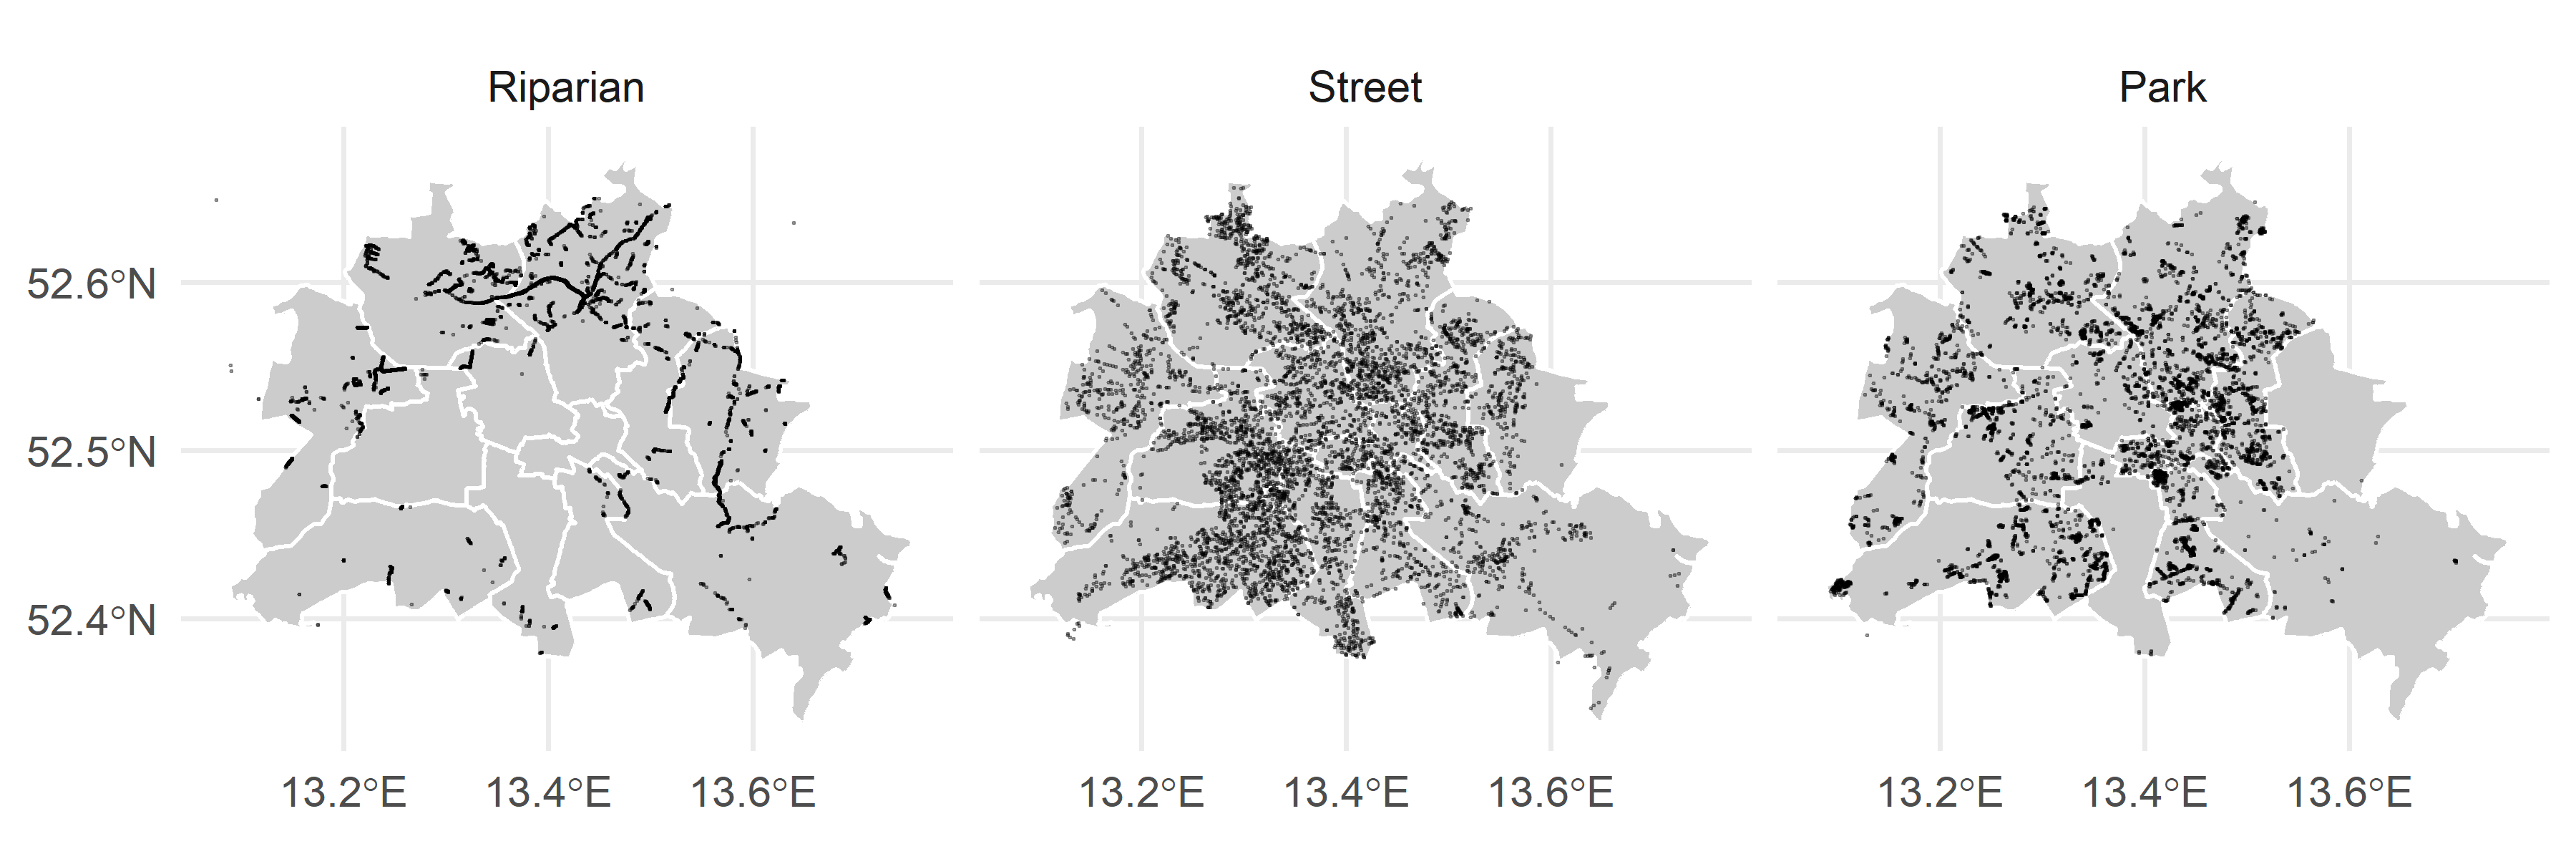
\includegraphics[width=1\linewidth]{C:/Users/ahurl/Documents/_work/p024_gfz_berlin-trees/berlin.trees/analysis/figures/map_01_overview} 

}

\caption{Individual tree locations for three categories available in Berlin Senate urban tree data set. Note, that for each category 7000 observations were subsampled from the available pool to facilitate visualization.}\label{fig:fig-tree-overview-map}
\end{figure}

\begin{figure}

{\centering 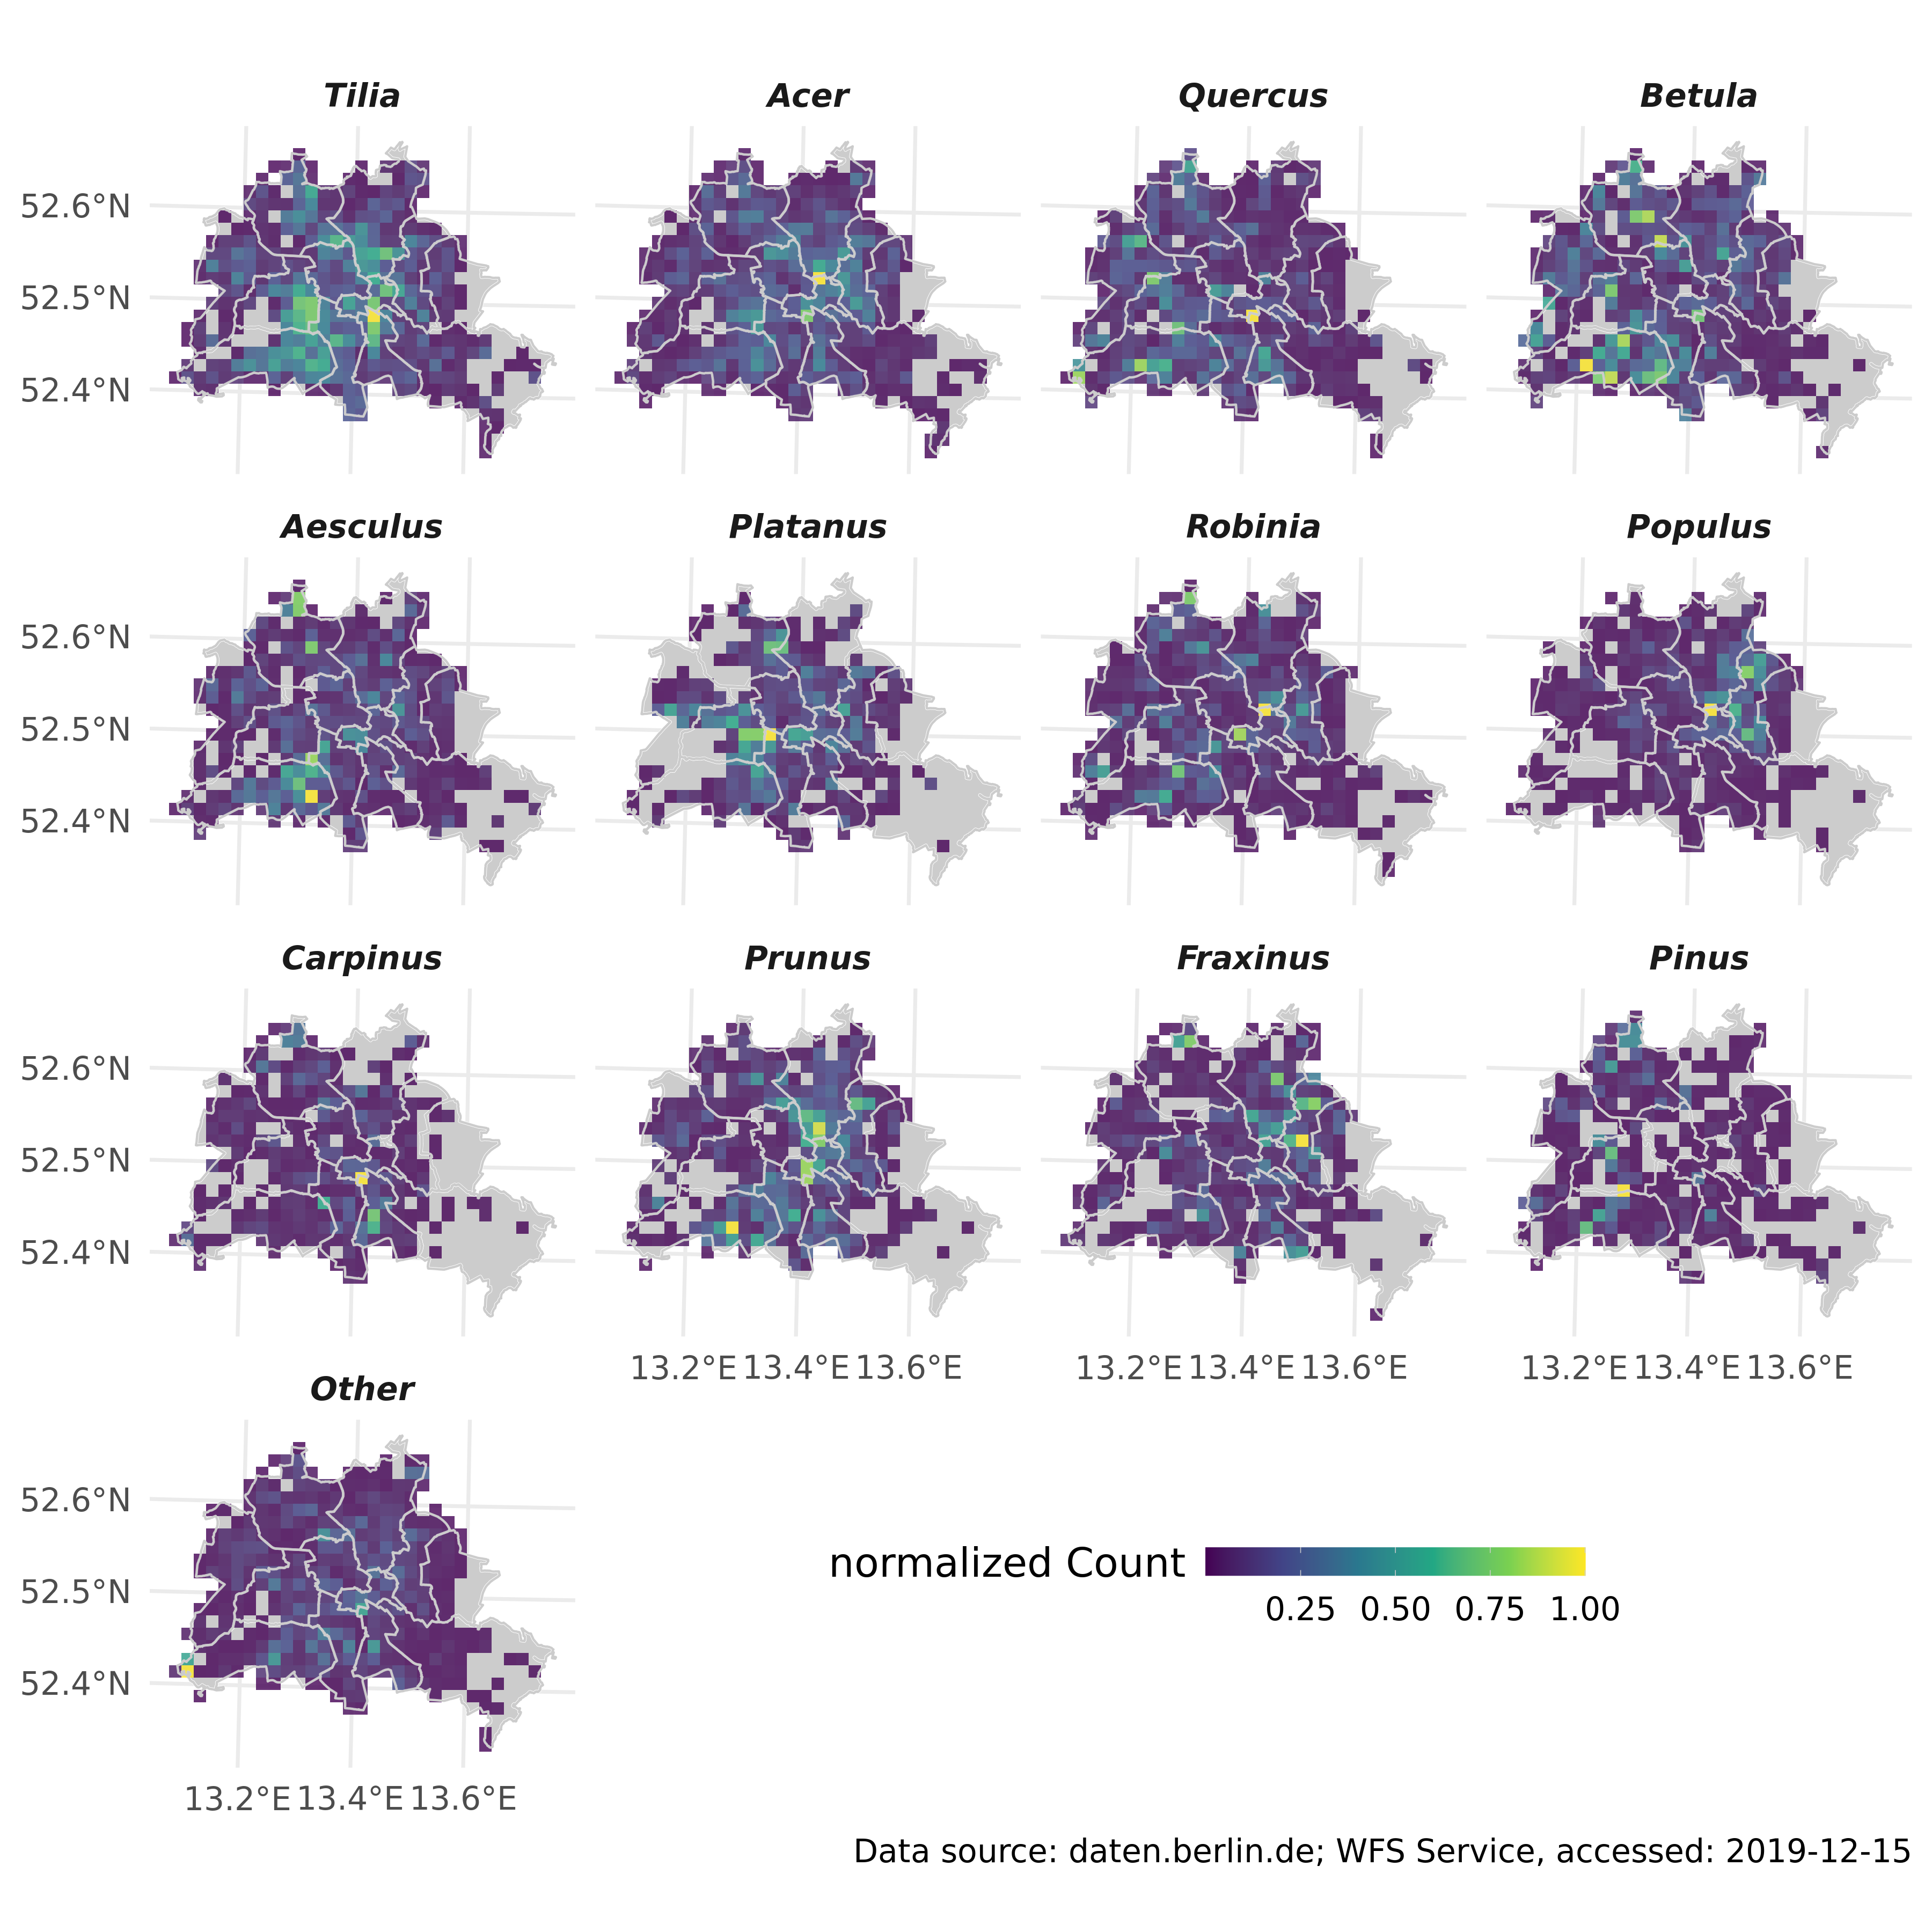
\includegraphics[width=1\linewidth]{C:/Users/ahurl/Documents/_work/p024_gfz_berlin-trees/berlin.trees/analysis/figures/map_02_tree_sums_standardized} 

}

\caption{Gridded counts for the 11 most frequent genera, as well as *Pinus* and remaining genera. Note, that counts are standardized to unity for individual genera.}\label{fig:fig-tree-count-map}
\end{figure}

The distribution of the UHI effect is highly irregular and clustered in space (Fig.\(~\)\ref{fig:fig-uhi-map}), and also shows variability through time (data not shown, refer to the \href{https://yceo.users.earthengine.app/view/uhimap}{urban heat island explorer}).



\begin{figure}

{\centering 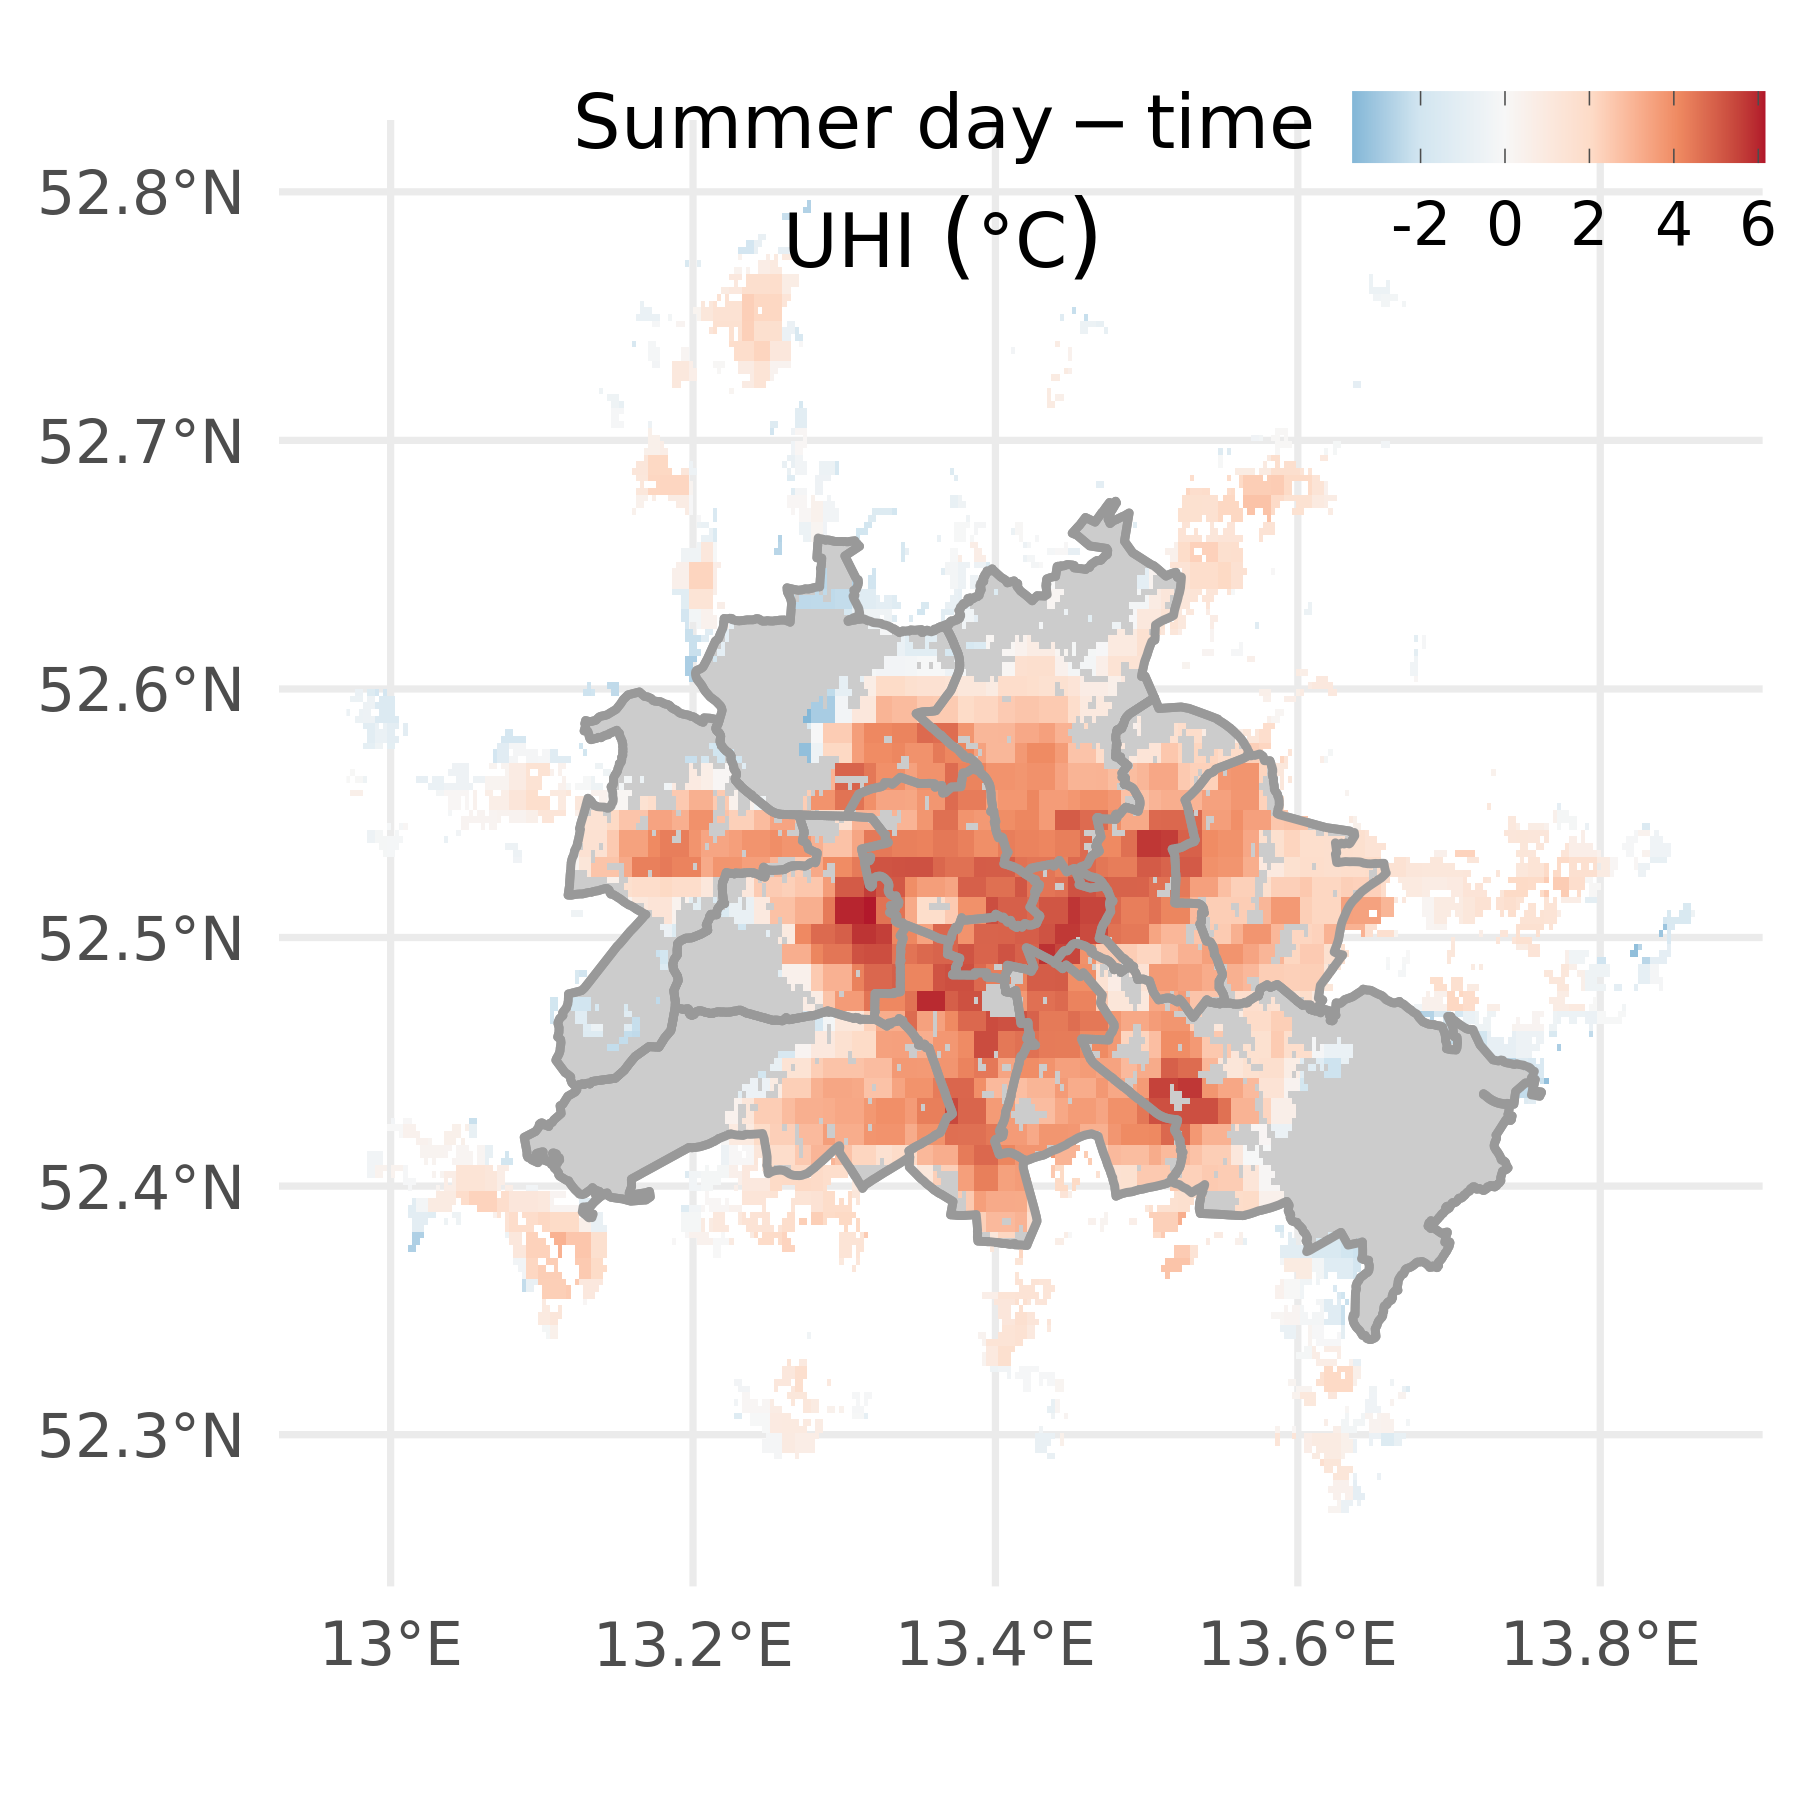
\includegraphics[width=0.5\linewidth]{C:/Users/ahurl/Documents/_work/p024_gfz_berlin-trees/berlin.trees/analysis/figures/map_03_uhi} 

}

\caption{Estimate of UHI intensity based on the algorithm in (Chakraborty and Lee, 2019), comparing urban with rural pixels within the greater metropolitan cluster. Presented values are averaged over the summer of 2007.}\label{fig:fig-uhi-map}
\end{figure}

The exposure to increased heat-loading of individual genera (and consequently species) is highly uneven throughout the city (Fig.\(~\)\ref{fig:fig-density}).
Street and park trees of most genera are clustered in urban areas with intermediate to high UHI loading, while riparian trees, and some street and park trees of other genera tend to be spread more evenly across Berlin's UHI range.

\begin{figure}

{\centering 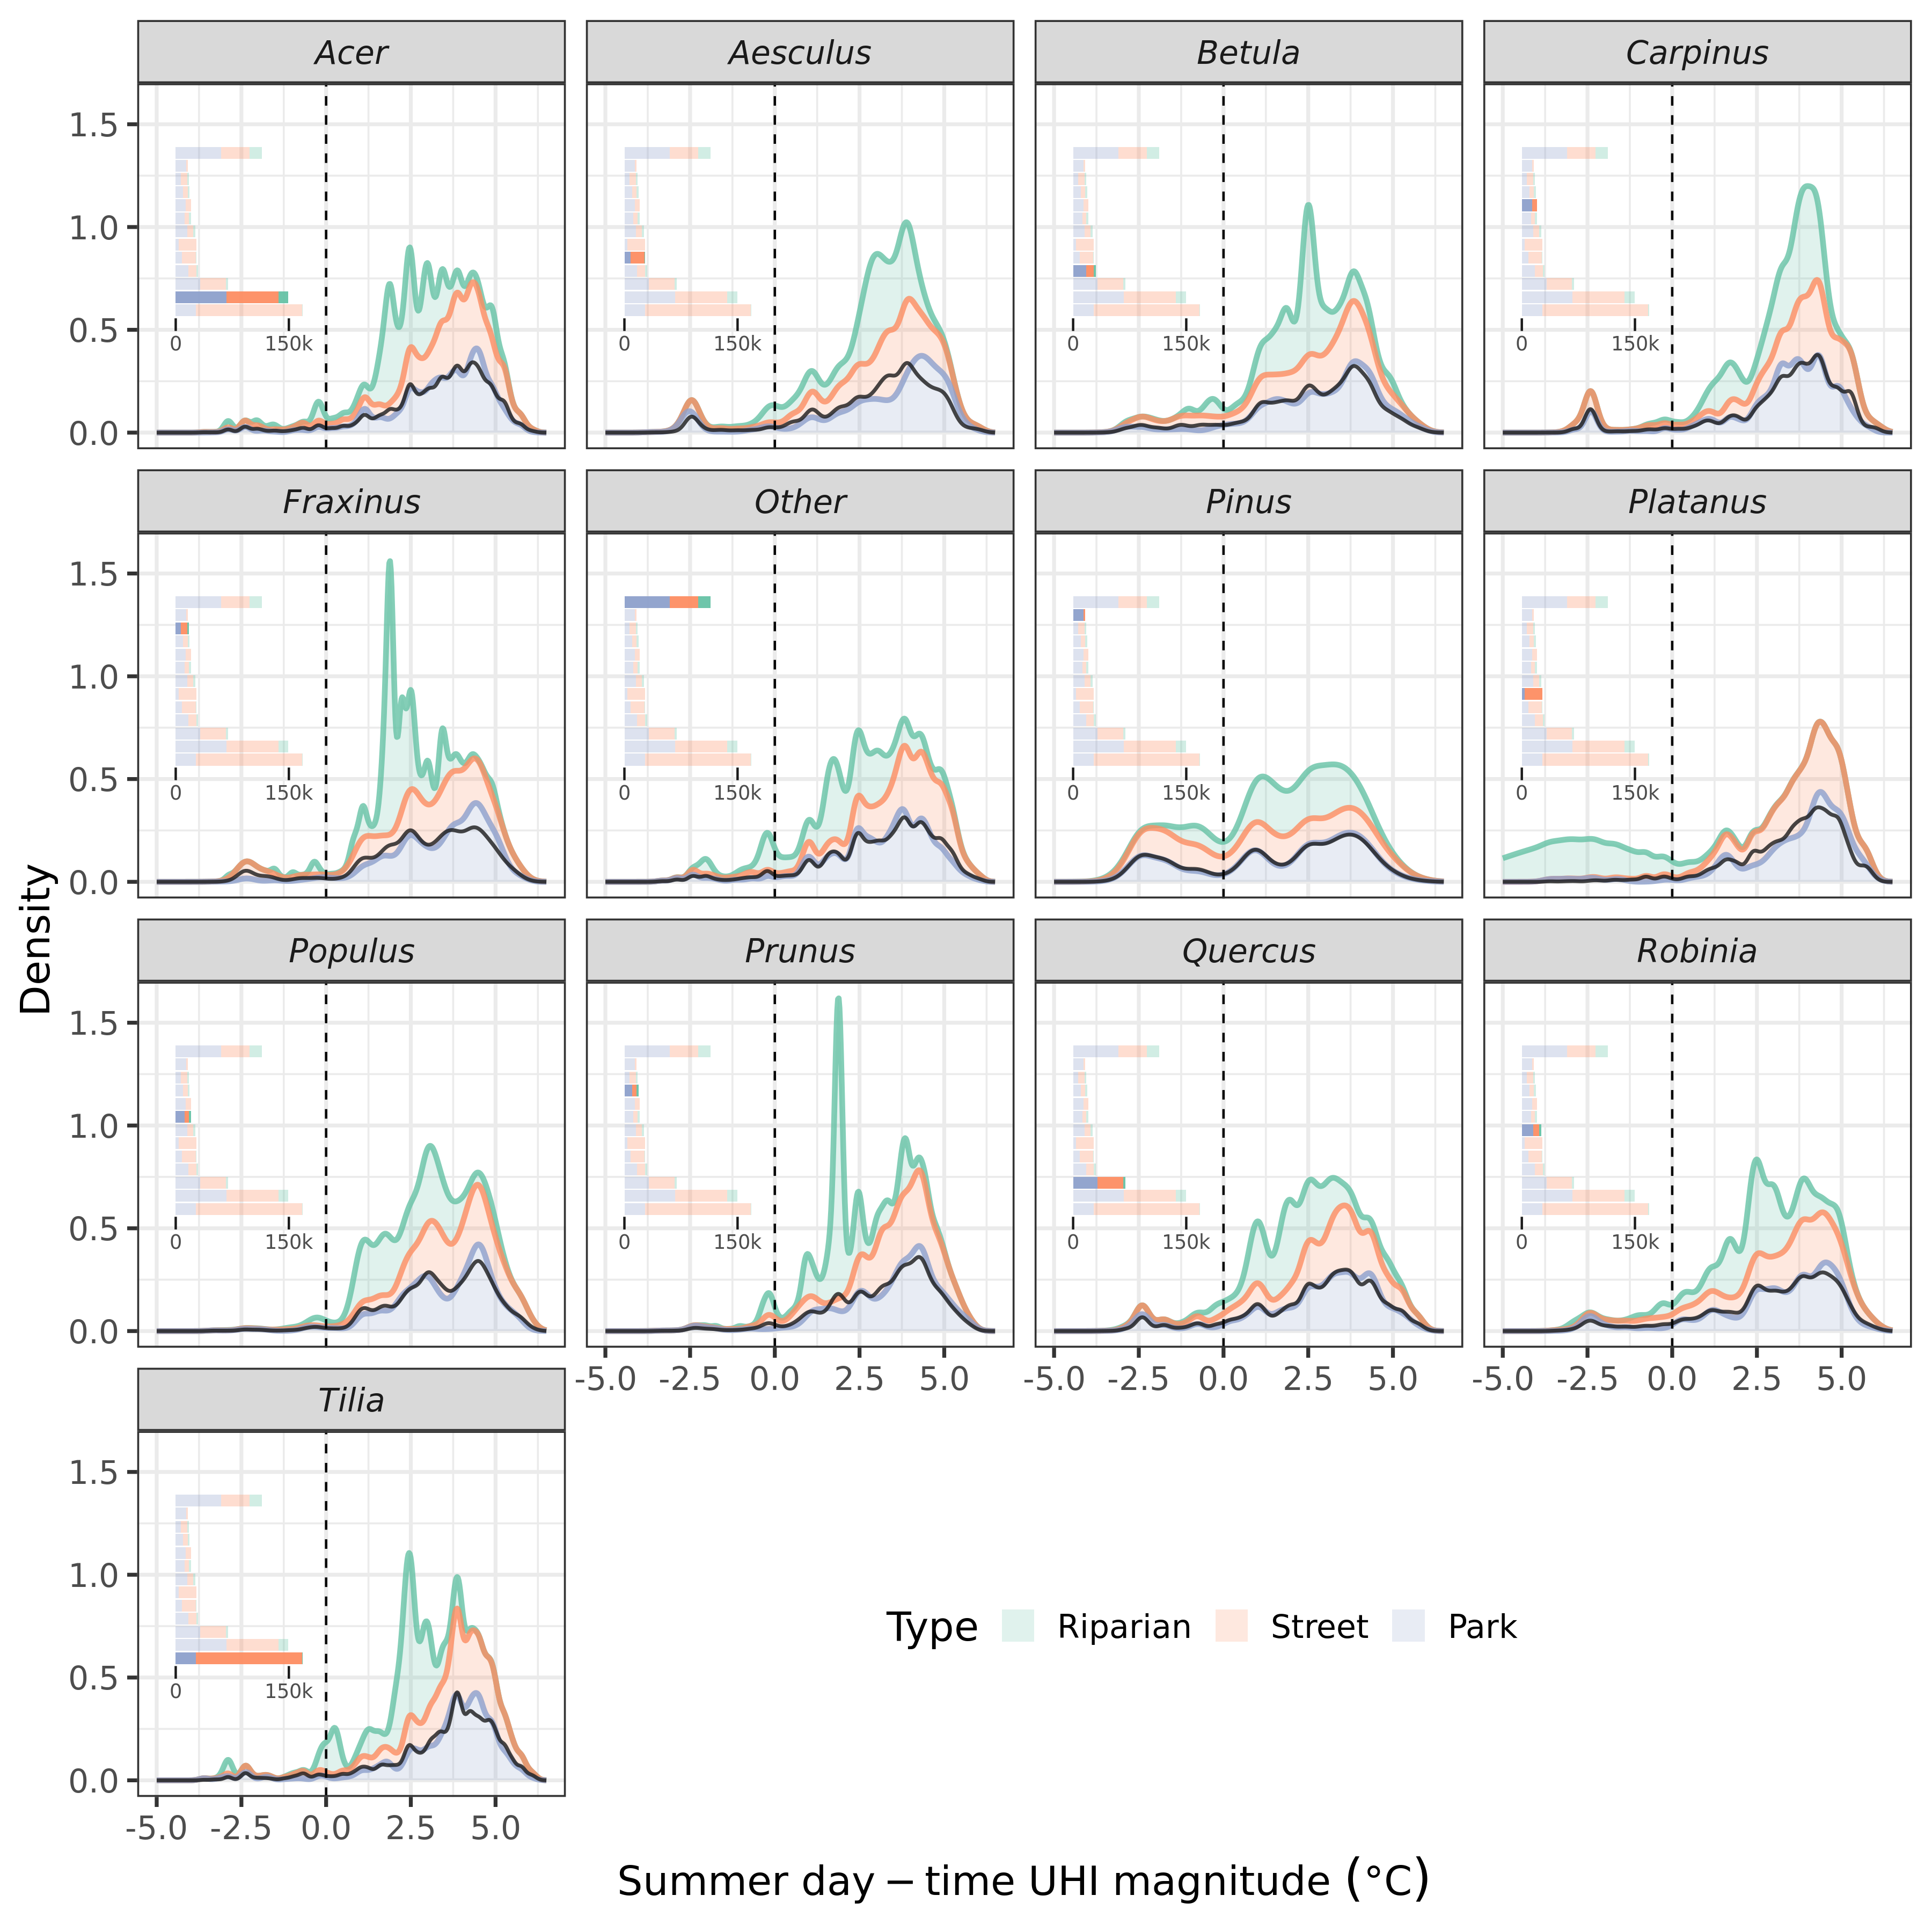
\includegraphics[width=1\linewidth]{C:/Users/ahurl/Documents/_work/p024_gfz_berlin-trees/berlin.trees/analysis/figures/plot_02_genus_UHI_dens} 

}

\caption{Empirical density distribution of all individuals within the presented genera along the UHI continuum. UHI intensities were extracted for each tree location, and the distribution hence represents the first detailed overview of the exposure of Berlin's trees to urban heat loading. The black line is the density across all three categories. Insets show corresponding tree totals.}\label{fig:fig-density}
\end{figure}

\textbf{Note, that results below are preliminary and should be considered as a template for future outputs, rather than used for inference.}
The effect of UHI loading on absolute growth potential varies between genera and species (Fig.\(~\)\ref{fig:fig-lmestat}).
Most notably, \emph{Quercus}, the 3rd-most frequent genera, shows decreased absolute growth with increasing UHI loading,
while the most frequent genera, \emph{Tilia}, features contrasting relationships between species.
The estimated effect sizes presented here are linear.
However, temperature may exert a non-linear control on absolute growth and, hence, applying a method able to capture such dynamics may result in somewhat different effect sizes / behavior.
Additionally, if temperatures increase in the future under climate warming, any non-linear effects may become more enhanced, stressing the need for a more flexible model fit and structure (i.e.~using GAMM over linear models-).

\begin{figure}

{\centering 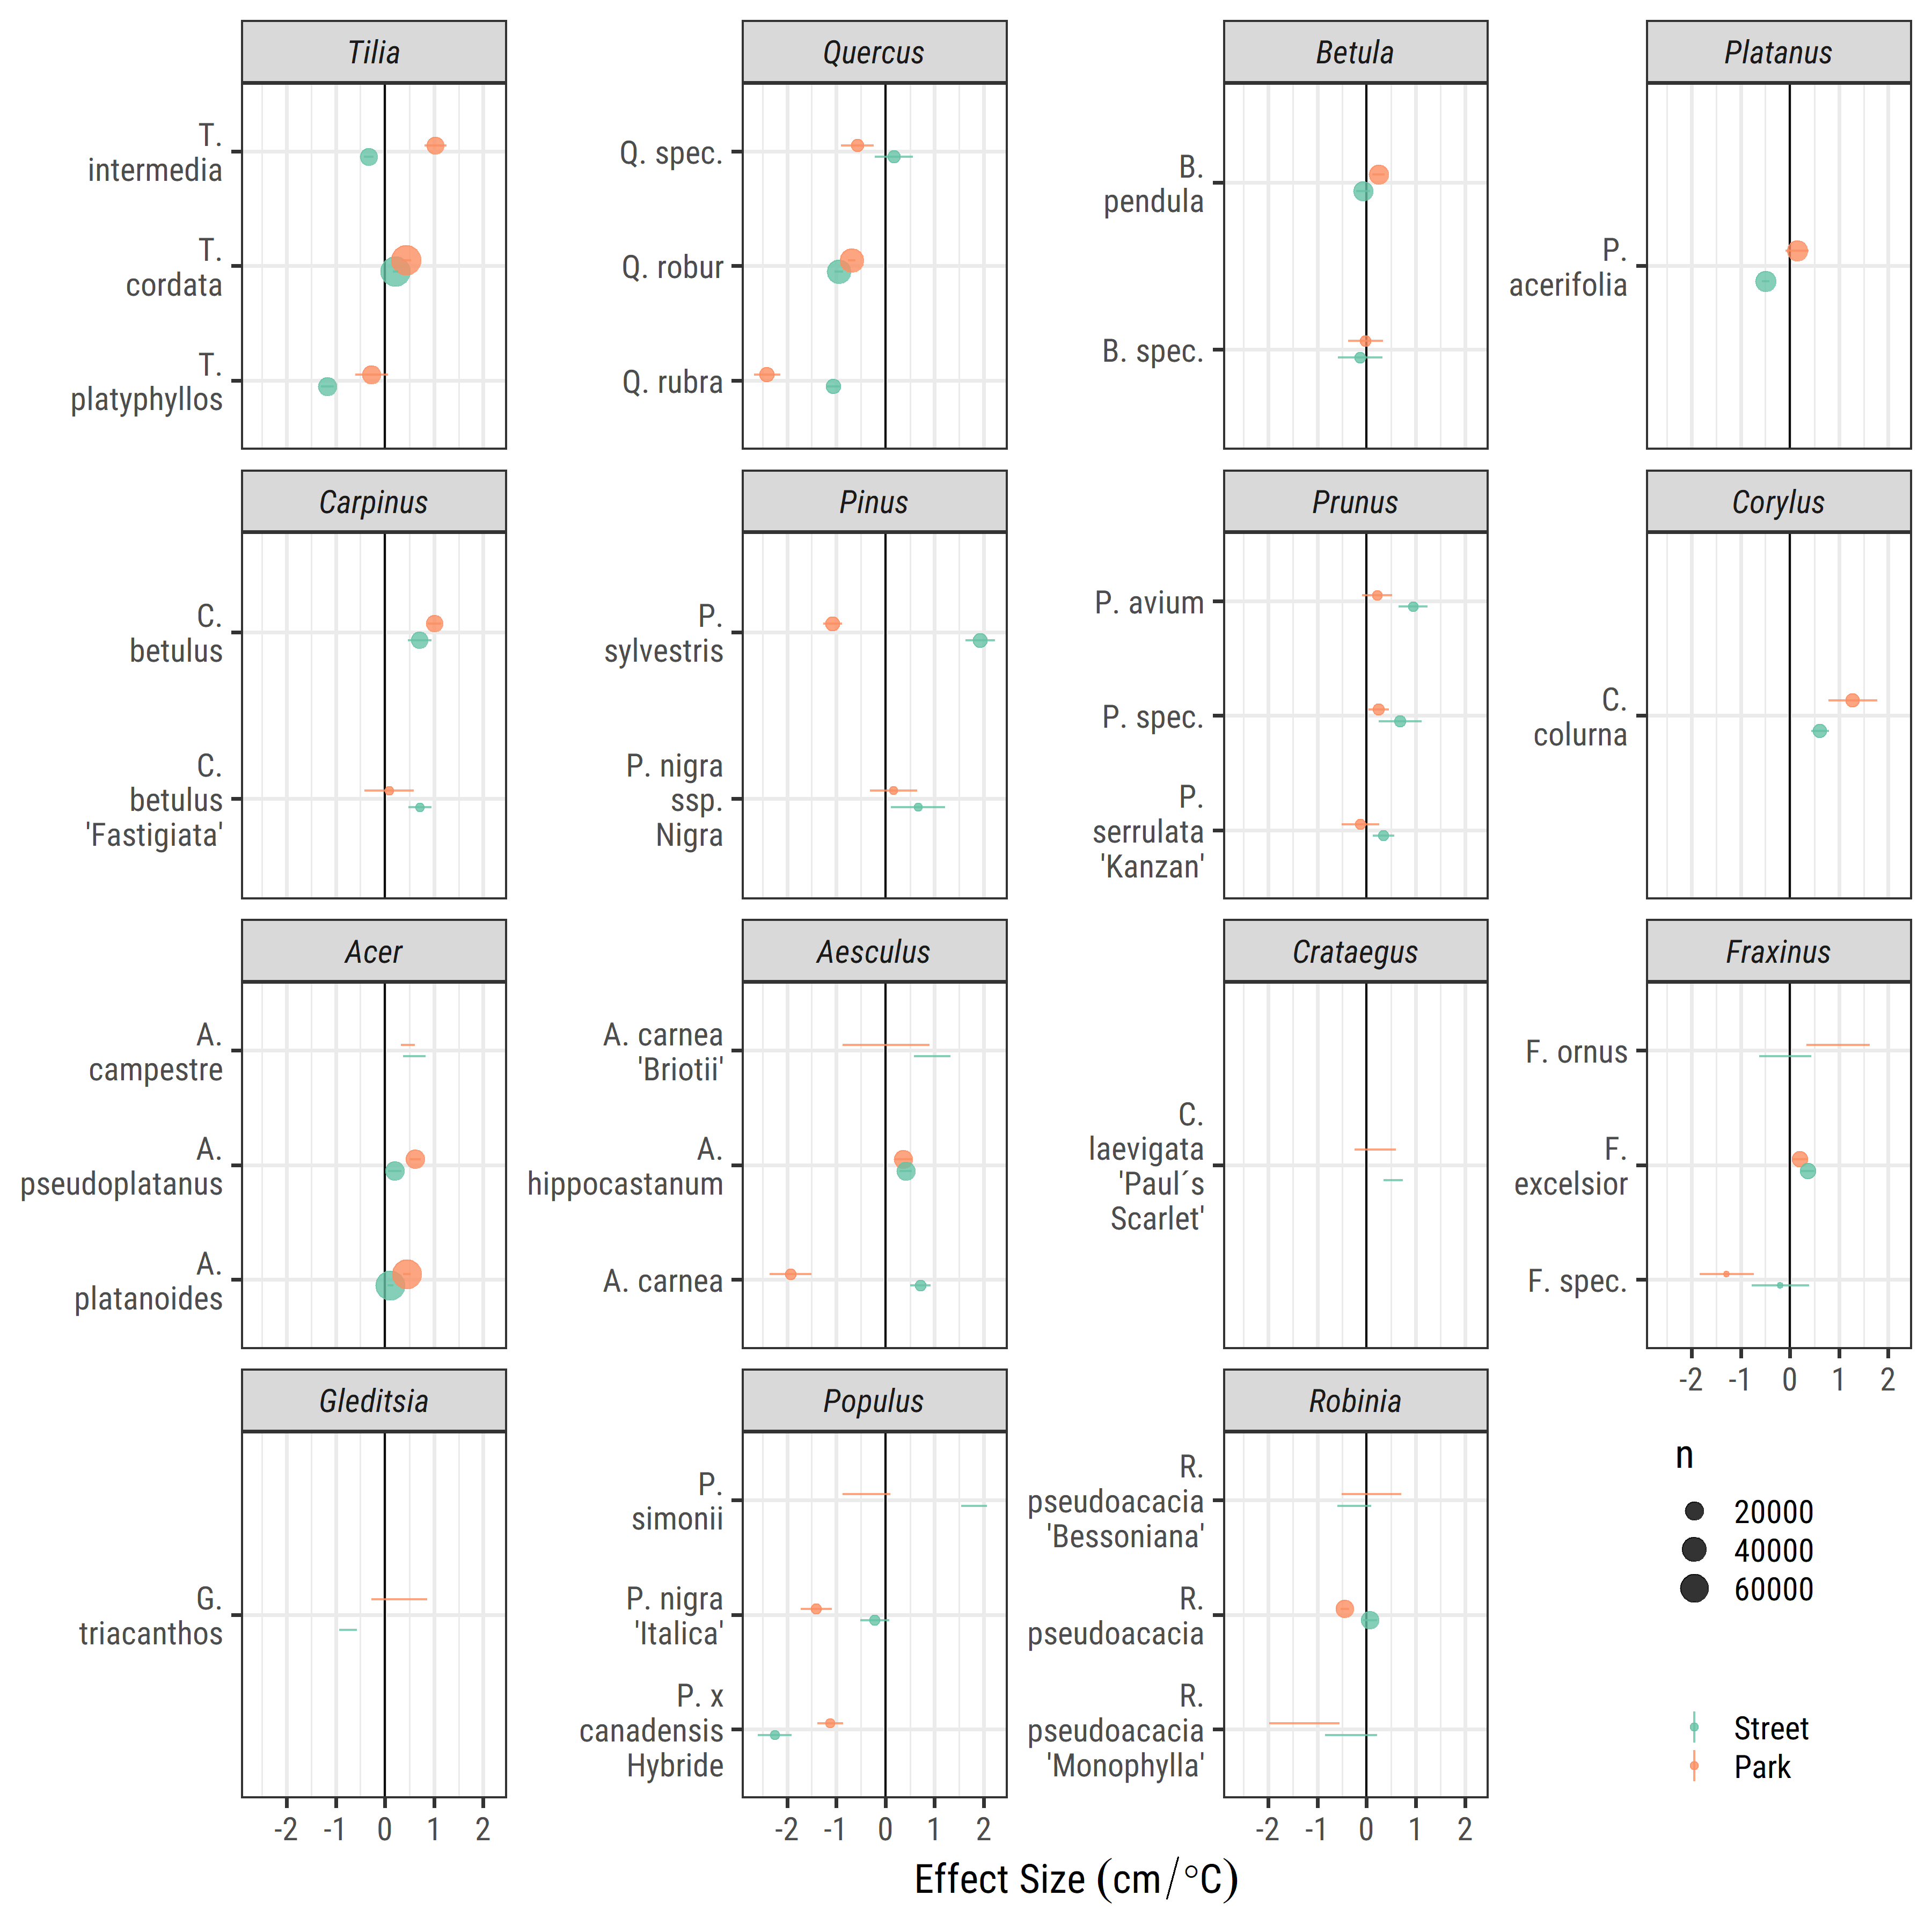
\includegraphics[width=1\linewidth]{C:/Users/ahurl/Documents/_work/p024_gfz_berlin-trees/berlin.trees/analysis/figures/plot_03_ranef_species_dbh_uhi} 

}

\caption{Impact of UHI loading on tree diameter (\(DBH\)), accounting for age and inter-specific differences from the linear mixed model (via random slopes and intercepts). Line-ranges are standard errors of predicted effect sizes (i.e. slopes). Differences between street and park trees are considerable for some species, and may be due to local clustering and/or spatial under-representation across the UHI continuum. Further investigations need to address the degree of spatial autocorrelation and account for it where required in linear mixed models, and with smoothing interactions in a GAMM implementation.}\label{fig:fig-lmestat}
\end{figure}

\hypertarget{outlook}{%
\section{Outlook}\label{outlook}}

We seek to build upon and improve the current analysis by:

\begin{itemize}
\tightlist
\item
  validating the database with independent observations
\item
  incorporating more pertinent covariates as dependent variables in the linear mixed model\\
\item
  testing multiple model structures with formal model selection procedures
\item
  checking model residuals for spatial auto-correlation and accounting for it where necessary to ensure unbiased estimates of effect sizes
\item
  repeating the above with a hierarchical GAM (i.e.~GAMM) to allow for:

  \begin{itemize}
  \tightlist
  \item
    estimating continuous prediction surfaces for UHI impacts on individual species' growth (similar to results in Figure\(~\)\ref{fig:fig-lmestat}) under recent conditions
  \item
    estimating absolute, species-specific growth potential under increased temperatures and UHI loading under climate change, ideally based on climate simulations (otherwise step-wise increases based on RCP scenarios) for the key species. Note, that complications presented by `out-of-sample' predictions will be addressed.
  \item
    assess potential age-dependent UHI impacts on individual species.\\
  \item
    repeating the above (GAMM) with total and incremental basal area as responses
  \end{itemize}
\end{itemize}

\hypertarget{references}{%
\section{References}\label{references}}

\hypertarget{refs}{}
\begin{CSLReferences}{1}{0}
\leavevmode\hypertarget{ref-akbari2001}{}%
Akbari, H., Pomerantz, M., Taha, H., 2001. Cool surfaces and shade trees to reduce energy use and improve air quality in urban areas. Solar Energy, Urban {Environment} 70, 295--310. \url{https://doi.org/10.1016/S0038-092X(00)00089-X}

\leavevmode\hypertarget{ref-akbari2001}{}%
Akbari, H., Pomerantz, M., Taha, H., 2001. Cool surfaces and shade trees to reduce energy use and improve air quality in urban areas. Solar Energy, Urban {Environment} 70, 295--310. \url{https://doi.org/10.1016/S0038-092X(00)00089-X}

\leavevmode\hypertarget{ref-augustin2009}{}%
Augustin, N.H., Musio, M., von Wilpert, K., Kublin, E., Wood, S.N., Schumacher, M., 2009. Modeling {Spatiotemporal Forest Health Monitoring Data}. Journal of the American Statistical Association 104, 899--911. \url{https://doi.org/10.1198/jasa.2009.ap07058}

\leavevmode\hypertarget{ref-augustin2009}{}%
Augustin, N.H., Musio, M., von Wilpert, K., Kublin, E., Wood, S.N., Schumacher, M., 2009. Modeling {Spatiotemporal Forest Health Monitoring Data}. Journal of the American Statistical Association 104, 899--911. \url{https://doi.org/10.1198/jasa.2009.ap07058}

\leavevmode\hypertarget{ref-bates2015}{}%
Bates, D., Mächler, M., Bolker, B., Walker, S., 2015. Fitting linear mixed-effects models using {lme4}. Journal of Statistical Software 67, 1--48. \url{https://doi.org/10.18637/jss.v067.i01}

\leavevmode\hypertarget{ref-bates2015}{}%
Bates, D., Mächler, M., Bolker, B., Walker, S., 2015. Fitting linear mixed-effects models using {lme4}. Journal of Statistical Software 67, 1--48. \url{https://doi.org/10.18637/jss.v067.i01}

\leavevmode\hypertarget{ref-beck2018}{}%
Beck, H.E., Zimmermann, N.E., McVicar, T.R., Vergopolan, N., Berg, A., Wood, E.F., 2018. Present and future {Köppen}-{Geiger} climate classification maps at 1-km resolution. Scientific Data 5, 180214. \url{https://doi.org/10.1038/sdata.2018.214}

\leavevmode\hypertarget{ref-brune2016}{}%
Brune, M., 2016. Urban trees under climate change. {Potential} impacts of dry spells and heat waves in three {German} regions in the 2050s (No. Report 24). {Climate Service Center Germany}, {Hamburg}.

\leavevmode\hypertarget{ref-brune2016}{}%
Brune, M., 2016. Urban trees under climate change. {Potential} impacts of dry spells and heat waves in three {German} regions in the 2050s (No. Report 24). {Climate Service Center Germany}, {Hamburg}.

\leavevmode\hypertarget{ref-chakraborty2019}{}%
Chakraborty, T., Lee, X., 2019. A simplified urban-extent algorithm to characterize surface urban heat islands on a global scale and examine vegetation control on their spatiotemporal variability. International Journal of Applied Earth Observation and Geoinformation 74, 269--280. \url{https://doi.org/10.1016/j.jag.2018.09.015}

\leavevmode\hypertarget{ref-chakraborty2019}{}%
Chakraborty, T., Lee, X., 2019. A simplified urban-extent algorithm to characterize surface urban heat islands on a global scale and examine vegetation control on their spatiotemporal variability. International Journal of Applied Earth Observation and Geoinformation 74, 269--280. \url{https://doi.org/10.1016/j.jag.2018.09.015}

\leavevmode\hypertarget{ref-dahlhausen2018}{}%
Dahlhausen, J., Rötzer, T., Biber, P., Uhl, E., Pretzsch, H., 2018. Urban climate modifies tree growth in {Berlin}. Int J Biometeorol 62, 795--808. \url{https://doi.org/10.1007/s00484-017-1481-3}

\leavevmode\hypertarget{ref-dahlhausen2018}{}%
Dahlhausen, J., Rötzer, T., Biber, P., Uhl, E., Pretzsch, H., 2018. Urban climate modifies tree growth in {Berlin}. Int J Biometeorol 62, 795--808. \url{https://doi.org/10.1007/s00484-017-1481-3}

\leavevmode\hypertarget{ref-endlicher2016}{}%
Endlicher, W., Scherer, D., Büter, B., Kuttler, W., Mathey, J., Schneider, C., 2016. Stadtnatur fördert gutes {Stadtklima}, in: Ökosystemleistungen in Der {Stadt} -- {Gesundheit} Schützen Und {Lebensqualität} Erhöhen, 3.1. {TEEB DE. TU Berlin, UFZ Leipzig}, {Berlin, Leipzig}, pp. 51--63.

\leavevmode\hypertarget{ref-endlicher2016}{}%
Endlicher, W., Scherer, D., Büter, B., Kuttler, W., Mathey, J., Schneider, C., 2016. Stadtnatur fördert gutes {Stadtklima}, in: Ökosystemleistungen in Der {Stadt} -- {Gesundheit} Schützen Und {Lebensqualität} Erhöhen, 3.1. {TEEB DE. TU Berlin, UFZ Leipzig}, {Berlin, Leipzig}, pp. 51--63.

\leavevmode\hypertarget{ref-fenner2017}{}%
Fenner, D., Meier, F., Bechtel, B., Otto, M., Scherer, D., 2017. Intra and inter {`local climate zone'} variability of air temperature as observed by crowdsourced citizen weather stations in {Berlin}, {Germany}. metz 26, 525--547. \url{https://doi.org/10.1127/metz/2017/0861}

\leavevmode\hypertarget{ref-fenner2017}{}%
Fenner, D., Meier, F., Bechtel, B., Otto, M., Scherer, D., 2017. Intra and inter {`local climate zone'} variability of air temperature as observed by crowdsourced citizen weather stations in {Berlin}, {Germany}. metz 26, 525--547. \url{https://doi.org/10.1127/metz/2017/0861}

\leavevmode\hypertarget{ref-fenner2014}{}%
Fenner, D., Meier, F., Scherer, D., Polze, A., 2014. Spatial and temporal air temperature variability in {Berlin}, {Germany}, during the years 2001--2010. Urban Climate, {ICUC8}: {The} 8th {International Conference} on {Urban Climate} and the 10th {Symposium} on the {Urban Environment} 10, 308--331. \url{https://doi.org/10.1016/j.uclim.2014.02.004}

\leavevmode\hypertarget{ref-fenner2014}{}%
Fenner, D., Meier, F., Scherer, D., Polze, A., 2014. Spatial and temporal air temperature variability in {Berlin}, {Germany}, during the years 2001--2010. Urban Climate, {ICUC8}: {The} 8th {International Conference} on {Urban Climate} and the 10th {Symposium} on the {Urban Environment} 10, 308--331. \url{https://doi.org/10.1016/j.uclim.2014.02.004}

\leavevmode\hypertarget{ref-gillner2014}{}%
Gillner, S., Bräuning, A., Roloff, A., 2014. Dendrochronological analysis of urban trees: Climatic response and impact of drought on frequently used tree species. Trees 28, 1079--1093. \url{https://doi.org/10.1007/s00468-014-1019-9}

\leavevmode\hypertarget{ref-gillner2014}{}%
Gillner, S., Bräuning, A., Roloff, A., 2014. Dendrochronological analysis of urban trees: Climatic response and impact of drought on frequently used tree species. Trees 28, 1079--1093. \url{https://doi.org/10.1007/s00468-014-1019-9}

\leavevmode\hypertarget{ref-gillner2015}{}%
Gillner, S., Vogt, J., Tharang, A., Dettmann, S., Roloff, A., 2015. Role of street trees in mitigating effects of heat and drought at highly sealed urban sites. Landscape and Urban Planning 143, 33--42. \url{https://doi.org/10.1016/j.landurbplan.2015.06.005}

\leavevmode\hypertarget{ref-gillner2015}{}%
Gillner, S., Vogt, J., Tharang, A., Dettmann, S., Roloff, A., 2015. Role of street trees in mitigating effects of heat and drought at highly sealed urban sites. Landscape and Urban Planning 143, 33--42. \url{https://doi.org/10.1016/j.landurbplan.2015.06.005}

\leavevmode\hypertarget{ref-grimmond1996}{}%
Grimmond, C., Souch, C., Hubble, M., 1996. Influence of tree cover on summertime surface energy balance fluxes, {San Gabriel Valley}, {Los Angeles}. Clim. Res. 6, 45--57. \url{https://doi.org/10.3354/cr006045}

\leavevmode\hypertarget{ref-grimmond1996}{}%
Grimmond, C., Souch, C., Hubble, M., 1996. Influence of tree cover on summertime surface energy balance fluxes, {San Gabriel Valley}, {Los Angeles}. Clim. Res. 6, 45--57. \url{https://doi.org/10.3354/cr006045}

\leavevmode\hypertarget{ref-gulyas2006}{}%
Gulyás, Á., Unger, J., Matzarakis, A., 2006. Assessment of the microclimatic and human comfort conditions in a complex urban environment: {Modelling} and measurements. Building and Environment 41, 1713--1722. \url{https://doi.org/10.1016/j.buildenv.2005.07.001}

\leavevmode\hypertarget{ref-gulyas2006}{}%
Gulyás, Á., Unger, J., Matzarakis, A., 2006. Assessment of the microclimatic and human comfort conditions in a complex urban environment: {Modelling} and measurements. Building and Environment 41, 1713--1722. \url{https://doi.org/10.1016/j.buildenv.2005.07.001}

\leavevmode\hypertarget{ref-hertel2019}{}%
Hertel, D., Schlink, U., 2019. Decomposition of urban temperatures for targeted climate change adaptation. Environmental Modelling \& Software 113, 20--28. \url{https://doi.org/10.1016/j.envsoft.2018.11.015}

\leavevmode\hypertarget{ref-hertel2019}{}%
Hertel, D., Schlink, U., 2019. Decomposition of urban temperatures for targeted climate change adaptation. Environmental Modelling \& Software 113, 20--28. \url{https://doi.org/10.1016/j.envsoft.2018.11.015}

\leavevmode\hypertarget{ref-hoyano1988}{}%
Hoyano, A., 1988. Climatological uses of plants for solar control and the effects on the thermal environment of a building. Energy and Buildings 11, 181--199. \url{https://doi.org/10.1016/0378-7788(88)90035-7}

\leavevmode\hypertarget{ref-hoyano1988}{}%
Hoyano, A., 1988. Climatological uses of plants for solar control and the effects on the thermal environment of a building. Energy and Buildings 11, 181--199. \url{https://doi.org/10.1016/0378-7788(88)90035-7}

\leavevmode\hypertarget{ref-jia2018}{}%
Jia, W., Zhao, S., Liu, S., 2018. Vegetation growth enhancement in urban environments of the {Conterminous United States}. Global Change Biology 24, 4084--4094. \url{https://doi.org/10.1111/gcb.14317}

\leavevmode\hypertarget{ref-jia2018}{}%
Jia, W., Zhao, S., Liu, S., 2018. Vegetation growth enhancement in urban environments of the {Conterminous United States}. Global Change Biology 24, 4084--4094. \url{https://doi.org/10.1111/gcb.14317}

\leavevmode\hypertarget{ref-kuttler2015}{}%
Kuttler, W., Miethke, A., Dütemeyer, D., Barlag, A.-B. (Eds.), 2015. Das klima von essen = the climate of essen. {Westarp Wiss.}, {Hohenwarsleben}.

\leavevmode\hypertarget{ref-kuttler2015}{}%
Kuttler, W., Miethke, A., Dütemeyer, D., Barlag, A.-B. (Eds.), 2015. Das klima von essen = the climate of essen. {Westarp Wiss.}, {Hohenwarsleben}.

\leavevmode\hypertarget{ref-maras2016}{}%
Maras, I., Schmidt, T., Paas, B., Ziefle, M., Schneider, C., 2016. The impact of human-biometeorological factors on perceived thermal comfort in urban public places. https://doi.org/\url{http://dx.doi.org/10.18452/18162}

\leavevmode\hypertarget{ref-maras2016}{}%
Maras, I., Schmidt, T., Paas, B., Ziefle, M., Schneider, C., 2016. The impact of human-biometeorological factors on perceived thermal comfort in urban public places. https://doi.org/\url{http://dx.doi.org/10.18452/18162}

\leavevmode\hypertarget{ref-mayer1987}{}%
Mayer, H., Höppe, P., 1987. Thermal comfort of man in different urban environments. Theor Appl Climatol 38, 43--49. \url{https://doi.org/10.1007/BF00866252}

\leavevmode\hypertarget{ref-mayer1987}{}%
Mayer, H., Höppe, P., 1987. Thermal comfort of man in different urban environments. Theor Appl Climatol 38, 43--49. \url{https://doi.org/10.1007/BF00866252}

\leavevmode\hypertarget{ref-mohamed2017}{}%
Mohamed, M.A., 2017. Monitoring of {Temporal} and {Spatial Changes} of {Land Use} and {Land Cover} in {Metropolitan Regions} through {Remote Sensing} and {GIS}. NR 08, 353--369. \url{https://doi.org/10.4236/nr.2017.85022}

\leavevmode\hypertarget{ref-moser-reischl2019a}{}%
Moser-Reischl, A., Rahman, M.A., Pauleit, S., Pretzsch, H., Rötzer, T., 2019. Growth patterns and effects of urban micro-climate on two physiologically contrasting urban tree species. Landscape and Urban Planning 183, 88--99. \url{https://doi.org/10.1016/j.landurbplan.2018.11.004}

\leavevmode\hypertarget{ref-moser-reischl2019a}{}%
Moser-Reischl, A., Rahman, M.A., Pauleit, S., Pretzsch, H., Rötzer, T., 2019. Growth patterns and effects of urban micro-climate on two physiologically contrasting urban tree species. Landscape and Urban Planning 183, 88--99. \url{https://doi.org/10.1016/j.landurbplan.2018.11.004}

\leavevmode\hypertarget{ref-norton2015}{}%
Norton, B.A., Coutts, A.M., Livesley, S.J., Harris, R.J., Hunter, A.M., Williams, N.S.G., 2015. Planning for cooler cities: {A} framework to prioritise green infrastructure to mitigate high temperatures in urban landscapes. Landscape and Urban Planning 134, 127--138. \url{https://doi.org/10.1016/j.landurbplan.2014.10.018}

\leavevmode\hypertarget{ref-norton2015}{}%
Norton, B.A., Coutts, A.M., Livesley, S.J., Harris, R.J., Hunter, A.M., Williams, N.S.G., 2015. Planning for cooler cities: {A} framework to prioritise green infrastructure to mitigate high temperatures in urban landscapes. Landscape and Urban Planning 134, 127--138. \url{https://doi.org/10.1016/j.landurbplan.2014.10.018}

\leavevmode\hypertarget{ref-oke1982}{}%
Oke, T.R., 1982. The energetic basis of the urban heat island. Quarterly Journal of the Royal Meteorological Society 108, 1--24. \url{https://doi.org/10.1002/qj.49710845502}

\leavevmode\hypertarget{ref-oke1982}{}%
Oke, T.R., 1982. The energetic basis of the urban heat island. Quarterly Journal of the Royal Meteorological Society 108, 1--24. \url{https://doi.org/10.1002/qj.49710845502}

\leavevmode\hypertarget{ref-pauleit2002}{}%
Pauleit, S., Jones, N., Garcia-Martin, G., Garcia-Valdecantos, J.L., Rivière, L.M., Vidal-Beaudet, L., Bodson, M., Randrup, T.B., 2002. Tree establishment practice in towns and cities -- {Results} from a {European} survey. Urban Forestry \& Urban Greening 1, 83--96. \url{https://doi.org/10.1078/1618-8667-00009}

\leavevmode\hypertarget{ref-pauleit2002}{}%
Pauleit, S., Jones, N., Garcia-Martin, G., Garcia-Valdecantos, J.L., Rivière, L.M., Vidal-Beaudet, L., Bodson, M., Randrup, T.B., 2002. Tree establishment practice in towns and cities -- {Results} from a {European} survey. Urban Forestry \& Urban Greening 1, 83--96. \url{https://doi.org/10.1078/1618-8667-00009}

\leavevmode\hypertarget{ref-pedersen2019}{}%
Pedersen, E.J., Miller, D.L., Simpson, G.L., Ross, N., 2019. Hierarchical generalized additive models in ecology: An introduction with mgcv. PeerJ 7, e6876. \url{https://doi.org/10.7717/peerj.6876}

\leavevmode\hypertarget{ref-pedersen2019}{}%
Pedersen, E.J., Miller, D.L., Simpson, G.L., Ross, N., 2019. Hierarchical generalized additive models in ecology: An introduction with mgcv. PeerJ 7, e6876. \url{https://doi.org/10.7717/peerj.6876}

\leavevmode\hypertarget{ref-pretzsch2017}{}%
Pretzsch, H., Biber, P., Uhl, E., Dahlhausen, J., Schütze, G., Perkins, D., Rötzer, T., Caldentey, J., Koike, T., Con, T. van, Chavanne, A., Toit, B. du, Foster, K., Lefer, B., 2017. Climate change accelerates growth of urban trees in metropolises worldwide. Scientific Reports 7, 1--10. \url{https://doi.org/10.1038/s41598-017-14831-w}

\leavevmode\hypertarget{ref-pretzsch2017}{}%
Pretzsch, H., Biber, P., Uhl, E., Dahlhausen, J., Schütze, G., Perkins, D., Rötzer, T., Caldentey, J., Koike, T., Con, T. van, Chavanne, A., Toit, B. du, Foster, K., Lefer, B., 2017. Climate change accelerates growth of urban trees in metropolises worldwide. Scientific Reports 7, 1--10. \url{https://doi.org/10.1038/s41598-017-14831-w}

\leavevmode\hypertarget{ref-quigley2004}{}%
Quigley, M.F., 2004. Street trees and rural conspecifics: {Will} long-lived trees reach full size in urban conditions? Urban Ecosystems 7, 29--39. \url{https://doi.org/10.1023/B:UECO.0000020170.58404.e9}

\leavevmode\hypertarget{ref-quigley2004}{}%
Quigley, M.F., 2004. Street trees and rural conspecifics: {Will} long-lived trees reach full size in urban conditions? Urban Ecosystems 7, 29--39. \url{https://doi.org/10.1023/B:UECO.0000020170.58404.e9}

\leavevmode\hypertarget{ref-rcoreteam2020}{}%
R Core Team, 2020. R: {A} language and environment for statistical computing. {R Foundation for Statistical Computing}, {Vienna, Austria}.

\leavevmode\hypertarget{ref-rcoreteam2020}{}%
R Core Team, 2020. R: {A} language and environment for statistical computing. {R Foundation for Statistical Computing}, {Vienna, Austria}.

\leavevmode\hypertarget{ref-randrup2001}{}%
Randrup, T.B., McPherson, E.G., Costello, L.R., 2001. A review of tree root conflicts with sidewalks, curbs, and roads. Urban Ecosystems 5, 209--225. \url{https://doi.org/10.1023/A:1024046004731}

\leavevmode\hypertarget{ref-randrup2001}{}%
Randrup, T.B., McPherson, E.G., Costello, L.R., 2001. A review of tree root conflicts with sidewalks, curbs, and roads. Urban Ecosystems 5, 209--225. \url{https://doi.org/10.1023/A:1024046004731}

\leavevmode\hypertarget{ref-rhoades1999}{}%
Rhoades, R.W., Stipes, R.J., 1999. Growth of trees on the {Virgina Tech Campus} in response to various factors 7.

\leavevmode\hypertarget{ref-rhoades1999}{}%
Rhoades, R.W., Stipes, R.J., 1999. Growth of trees on the {Virgina Tech Campus} in response to various factors 7.

\leavevmode\hypertarget{ref-roloff2009}{}%
Roloff, A., Korn, S., Gillner, S., 2009. The {Climate}-{Species}-{Matrix} to select tree species for urban habitats considering climate change. Urban Forestry \& Urban Greening 8, 295--308. \url{https://doi.org/10.1016/j.ufug.2009.08.002}

\leavevmode\hypertarget{ref-roloff2009}{}%
Roloff, A., Korn, S., Gillner, S., 2009. The {Climate}-{Species}-{Matrix} to select tree species for urban habitats considering climate change. Urban Forestry \& Urban Greening 8, 295--308. \url{https://doi.org/10.1016/j.ufug.2009.08.002}

\leavevmode\hypertarget{ref-suvkberlin2019}{}%
SUVK, Berlin, 2019. Anteil öffentlicher {Grünflächen} in {Berlin}, Grünflächeninformationssystem ({GRIS}). {Senatsverwaltung für Umwelt, Verkehr und Klimaschutz Berlin, Referat Freiraumplanung und Stadtgrün}, {Berlin}.

\leavevmode\hypertarget{ref-tzoulas2007}{}%
Tzoulas, K., Korpela, K., Venn, S., Yli-Pelkonen, V., Kaźmierczak, A., Niemela, J., James, P., 2007. Promoting ecosystem and human health in urban areas using {Green Infrastructure}: {A} literature review. Landscape and Urban Planning 81, 167--178. \url{https://doi.org/10.1016/j.landurbplan.2007.02.001}

\leavevmode\hypertarget{ref-tzoulas2007}{}%
Tzoulas, K., Korpela, K., Venn, S., Yli-Pelkonen, V., Kaźmierczak, A., Niemela, J., James, P., 2007. Promoting ecosystem and human health in urban areas using {Green Infrastructure}: {A} literature review. Landscape and Urban Planning 81, 167--178. \url{https://doi.org/10.1016/j.landurbplan.2007.02.001}

\leavevmode\hypertarget{ref-wood2017}{}%
Wood, S.N., 2017. Generalized additive models: An introduction with {R}. {CRC press}.

\leavevmode\hypertarget{ref-wood2017}{}%
Wood, S.N., 2017. Generalized additive models: An introduction with {R}. {CRC press}.

\leavevmode\hypertarget{ref-zhao2016}{}%
Zhao, S., Liu, S., Zhou, D., 2016. Prevalent vegetation growth enhancement in urban environment. PNAS 113, 6313--6318. \url{https://doi.org/10.1073/pnas.1602312113}

\leavevmode\hypertarget{ref-zhao2016}{}%
Zhao, S., Liu, S., Zhou, D., 2016. Prevalent vegetation growth enhancement in urban environment. PNAS 113, 6313--6318. \url{https://doi.org/10.1073/pnas.1602312113}

\end{CSLReferences}

\newpage

\hypertarget{colophon}{%
\subsubsection{Colophon}\label{colophon}}

This report was generated on 2021-05-18 14:55:27 using the following computational environment and dependencies:

The current Git commit details are:

\begin{verbatim}
#> Local:    master C:/Users/ahurl/Documents/_work/p024_gfz_berlin-trees/berlin.trees
#> Remote:   master @ origin (https://github.com/the-Hull/berlin.trees.git)
#> Head:     [43beb0c] 2021-05-18: add refs
\end{verbatim}

\end{document}
